\documentclass{article}
\usepackage{fullpage}
\usepackage[utf8]{inputenc}
\usepackage{pict2e}
\usepackage{amsmath}
\usepackage{enumitem}
\usepackage{eurosym}
\usepackage{mathtools}
\usepackage{amssymb, amsfonts, latexsym, cancel}
\setlength{\parskip}{0.3cm}
\usepackage{graphicx}
\usepackage{fontenc}
\usepackage{slashbox}
\usepackage{setspace}
\usepackage{gensymb}
\usepackage{accents}
\usepackage{adjustbox}
\setstretch{1.35}
\usepackage{bold-extra}
\usepackage[document]{ragged2e}
\usepackage{subcaption}
\usepackage{tcolorbox}
\usepackage{xcolor, colortbl}
\usepackage{wrapfig}
\usepackage{empheq}
\usepackage{array}
\usepackage{parskip}
\usepackage{arydshln}
\graphicspath{ {images/} }
\renewcommand*\contentsname{\color{black}Índice} 
\usepackage{array, multirow, multicol}
\definecolor{lightblue}{HTML}{007AFF}
\usepackage{color}
\usepackage{etoolbox}
\usepackage{listings}
\usepackage{mdframed}
\setlength{\parindent}{0pt}
\usepackage{underscore}
\usepackage{hyperref}
\usepackage{tikz}
\usepackage{tikz-cd}
\usetikzlibrary{shapes, positioning, patterns}
\usepackage{tikz-qtree}
\usepackage{biblatex}
\usepackage{pdfpages}
\usepackage{pgfplots}
\usepackage{pgfkeys}
\addbibresource{biblatex-examples.bib}
\usepackage[a4paper, left=1cm, right=1cm, top=1cm,
bottom=1.5cm]{geometry}
\usepackage{titlesec}
\usepackage{titletoc}
\usepackage{tikz-3dplot}
\usepackage{kbordermatrix}
\usetikzlibrary{decorations.pathreplacing}
\newcommand{\Ej}{\textcolor{lightblue}{\underline{Ejemplo}}}
\setlength{\fboxrule}{1.5pt}

% Configura el formato de las secciones utilizando titlesec
\titleformat{\section}
{\color{red}\normalfont\LARGE\bfseries}
{Tema \thesection:}
{10 pt}
{}

% Ajusta el formato de las entradas de la tabla de contenidos
\addtocontents{toc}{\protect\setcounter{tocdepth}{4}}
\addtocontents{toc}{\color{black}}

\titleformat{\subsection}
{\normalfont\Large\bfseries\color{red}}{\thesubsection)}{1em}{\color{lightblue}}

\titleformat{\subsubsection}
{\normalfont\large\bfseries\color{red}}{\thesubsubsection)}{1em}{\color{lightblue}}

\newcommand{\bboxed}[1]{\fcolorbox{lightblue}{lightblue!10}{$#1$}}
\newcommand{\rboxed}[1]{\fcolorbox{red}{red!10}{$#1$}}

\DeclareMathOperator{\N}{\mathbb{N}}
\DeclareMathOperator{\Z}{\mathbb{Z}}
\DeclareMathOperator{\R}{\mathbb{R}}
\DeclareMathOperator{\Q}{\mathbb{Q}}
\DeclareMathOperator{\K}{\mathbb{K}}
\DeclareMathOperator{\im}{\imath}
\DeclareMathOperator{\jm}{\jmath}
\DeclareMathOperator{\col}{\mathrm{Col}}
\DeclareMathOperator{\fil}{\mathrm{Fil}}
\DeclareMathOperator{\rg}{\mathrm{rg}}
\DeclareMathOperator{\nuc}{\mathrm{nuc}}
\DeclareMathOperator{\dimf}{\mathrm{dimFil}}
\DeclareMathOperator{\dimc}{\mathrm{dimCol}}
\DeclareMathOperator{\dimn}{\mathrm{dimnuc}}
\DeclareMathOperator{\dimr}{\mathrm{dimrg}}
\DeclareMathOperator{\dom}{\mathrm{Dom}}
\DeclareMathOperator{\infi}{\int_{-\infty}^{+\infty}}
\newcommand{\dint}[2]{\int_{#1}^{#2}}

\newcommand{\bu}[1]{\textcolor{lightblue}{\underline{#1}}}
\newcommand{\lb}[1]{\textcolor{lightblue}{#1}}
\newcommand{\db}[1]{\textcolor{blue}{#1}}
\newcommand{\rc}[1]{\textcolor{red}{#1}}
\newcommand{\tr}{^\intercal}

\renewcommand{\CancelColor}{\color{lightblue}}

\newcommand{\dx}{\:\mathrm{d}x}
\newcommand{\dt}{\:\mathrm{d}t}
\newcommand{\dy}{\:\mathrm{d}y}
\newcommand{\dz}{\:\mathrm{d}z}
\newcommand{\dth}{\:\mathrm{d}\theta}
\newcommand{\dr}{\:\mathrm{d}\rho}
\newcommand{\du}{\:\mathrm{d}u}
\newcommand{\dv}{\:\mathrm{d}v}
\newcommand{\tozero}[1]{\cancelto{0}{#1}}
\newcommand{\lbb}[2]{\textcolor{lightblue}{\underbracket[1pt]{\textcolor{black}{#1}}_{#2}}}
\newcommand{\dbb}[2]{\textcolor{blue}{\underbracket[1pt]{\textcolor{black}{#1}}_{#2}}}
\newcommand{\rub}[2]{\textcolor{red}{\underbracket[1pt]{\textcolor{black}{#1}}_{#2}}}

\author{Francisco Javier Mercader Martínez}
\date{}
\title{Fundamentos de Inferencia Estadística}
\usepackage{hyperref}
\usepackage{float}
\usepackage{varwidth}
\lstset{
    language=R,
    basicstyle=\ttfamily\small,
    keywordstyle=\color{blue},
    commentstyle=\color{green!70!black}\itshape,
    stringstyle=\color{red},
    showstringspaces=false,
    breaklines=true,
    numbers=left,
    numberstyle=\tiny,
    stepnumber=1,
    numbersep=5pt,
    frame=single,
    backgroundcolor=\color{lightgray!10},
    captionpos=b,
    tabsize=2,
    inputencoding=utf8,
    literate={á}{{\'a}}1 {é}{{\'e}}1 {í}{{\'i}}1 {ó}{{\'o}}1 {ú}{{\'u}}1{ñ}{{\~n}}1,
    mathescape=false
}
\begin{document}

\thispagestyle{empty}

\maketitle

\tableofcontents
\thispagestyle{empty}

\newpage
\setcounter{page}{1}
\section{Vectores aleatorios}

\subsection{Introducción}

\lb{Objetivo: }estudiar $k$ variables sobre una población de individuos (objetos).

\lb{Algunos ejemplos:}
\begin{itemize}[label=$\to$]
\item Las variables meteorológicas como temperatura, humedad y velocidad del viento.
\item La intensidad y la fase de una señal aleatoria que se miden en los canales de comunicación.
\item Los parámetros clínicos de los pacientes (como presión arterial, niveles de glucosa, etc.)
\end{itemize}
Habitualmente estas variables cualitativas o discretas que nos indicarán grupos de individuos.

Estas variables se representarán mediante vectores aleatorios sobre un espacio de probabilidad.

\begin{enumerate}[label=\arabic*)]
	\item Definiciones
\end{enumerate}

Un \lb{vector aleatorio} (v.a.) $k$-dimensional sobre un espacio de probabilidad $(\Omega,\mathcal{S},\mathcal{P})$ es $X=(X_1,\dots,X_k)$ tal que \[ X_i^{-1}(-\infty,x]\in\mathcal{S} \]para todo $x\in\R,\, i=1,\dots,k$

\begin{itemize}[label=\color{red}\textbullet, leftmargin=*]
	\item \color{lightblue}Función de distribución conjunta
\end{itemize}

$F:\R^k\longrightarrow[0,1],$\[ F(x_1,\dots,x_k)\coloneq P[X_1\le x_1,X_2\le x_2,\dots,X_k\le x_k], \] para todo $x_1,\dots,x_k\in\R$.

\subsection{Independencia de las variables aleatorias}

\begin{itemize}[label=\color{red}\textbullet, leftmargin=*]
	\item \color{lightblue}Definición
\end{itemize}
Las variables aleatorias $X_1,\dots,X_k$ son \lb{independientes} si los sucesos \[ \{x_1\le x_1\},\{X_2\le x_2\},\dots,\{X_k\le x_k\} \]son independientes para todo $x_1,\dots,x_k\in\R$.

Esto es equivalente a que \[ F(x_1,\dots,x_k)=P[X_1\le x_1]\cdot P[X_2\le x_2]\cdots P[X_k\le x_k] \]para todo $x_1,\dots,x_k\in\R$.


\subsection{Distribuciones marginales}

La función $F_{X_i}(x_i)=P[X_i\le x_i]$ se denomina \lb{función de distribución marginal} $i$-ésima y corresponde con la función de distribución de la variable aleatoria $X_i$

Las \lb{distribuciones marginales} pueden obtenerse a partir de la distribución conjunta: \[ F_{X_i}(x_I)=F(+\infty,\dots,+\infty,x_i,+\infty,\dots,+\infty) \]
Análogamente, la \lb{función de distribución marginal del subvector aleatorio} $(X_{i_1},\dots,X_{i_m})$ vendrá dada por \[ F_{X_{i_1},\dots,X_{i_m}}(x_{i_1},\dots,x_{i_m})=F(+\infty,\dots,+\infty,x_{i_1},+\infty,\dots,+\infty,x_{i_m},+\infty,\dots,+\infty). \]

\subsection{Vector aleatorio absolutamente continuo}

Un \vea $X$ es \lb{absolutamente continuo} si existe una función $f:\R^k\longrightarrow\R$ no negativa (llamada \lb{función de densidad}) tal que \[ F(x)=F(x_1,\dots,x_k)=\int_{-\infty}^{x_1}\cdots\int_{-\infty}^{x_k}f(z_1,\dots,z_k)\mathrm{d}z_k,\dots,\mathrm{d}z_1, \]para todo $x=(x_1,\dots,x_k)\in\R^k$

Usando el \lb{teorema fundamental del cálculo}, se tiene que en cada punto de continuidad $(x_1,\dots,x_k)$ de $f$: \[ \dfrac{\partial^kF(x_1,\dots,x_k)}{\partial x_1,\dots,\partial x_k}=f(x_1,\dots,x_k).\]

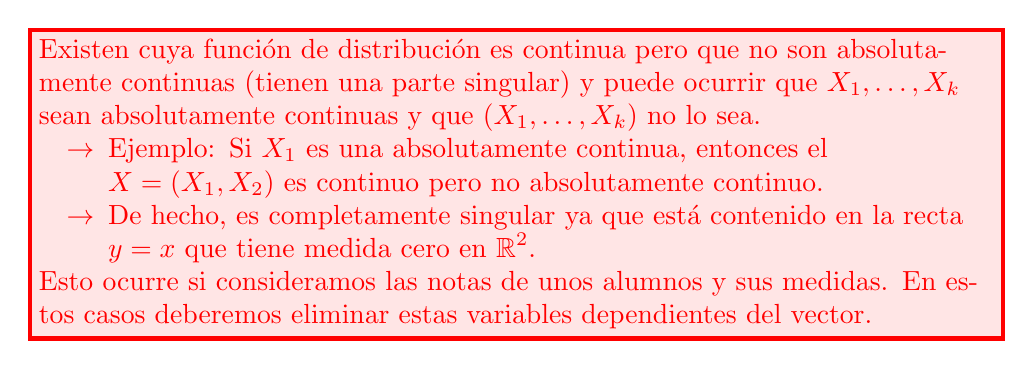
\begin{tikzpicture}
	\node[red, draw=red, fill=red!10, line width=1.5, text width=\textwidth] {Existen \vas cuya función de distribución es continua pero que no son absolutamente continuas (tienen una parte singular) y puede ocurrir que $X_1,\dots,X_k$ sean absolutamente continuas y que $(X_1,\dots,X_k)$ no lo sea.
	\begin{itemize}[label=$\to$]
	\item Ejemplo: Si $X_1$ es una \va absolutamente continua, entonces el \vea $X=(X_1,X_2)$ es continuo pero no absolutamente continuo.
	
	\item De hecho, es completamente singular ya que está contenido en la recta $y=x$ que tiene medida cero en $\R^2$.
	\end{itemize}
	Esto ocurre si consideramos las notas de unos alumnos y sus medidas. En estos casos deberemos eliminar estas variables dependientes del vector.
	};
\end{tikzpicture}

\subsection{Vector aleatorio discreto}
Un vector aleatorio $X$ se dice que es \lb{discreto} si existe un conjunto numerable $\mathcal{S}\in\R^k$ tal que $P(X\in\mathcal{S})=1$.

\lb{Función masa de probabilidad} de una vector aleatorio discreto: \[ P[X=x]=P[X_1=x_1,\dots,X_k=x_k] \]para todo $x=(x_1,\dots,x_k)\in\R^k$, satisfaciendo:
\begin{itemize}[label=$\to$]
\item $P[X=x]\ge0,\;\forall x\in\mathcal{S}$
\item $\sum_{x\in\mathcal{S}}P[X=x]=1$
\end{itemize}
\lb{Función de distribución} de un \vea discreto: \[ F(x)=P[X\le x]=\sum_{\begin{subarray}{c}
z\in\mathcal{S}\\
z\le x
\end{subarray}}P[X=z], \]para todo $x\in\R^k$.

\subsection{Distribuciones marginales}
\subsubsection{Caso continuo}
\begin{itemize}[label=\color{red}\textbullet, leftmargin=*]
	\item \color{lightblue}Distribución marginal de la variable aleatoria $X_i$
\end{itemize}
Sea $X=(X_1,\dots,X_k)$ un \vea continuo con función de densidad $f$ entonces cada componente $X_i$ es de tipo continuo y su función de distribución es; \[ F_{X_i}(x_i)=P[X_i\le x_i]=\int_{-\infty}^{x_i}f_{X_i}(z_i)\mathrm{d}z_i, \]con\[ f_{X_i}=\int_{-\infty}^{+\infty}\cdots\int_{-\infty}^{+\infty}f(z_1,\dots,z_k)\mathrm{d}z_1,\dots,\mathrm{d}z_{i-1}\cdot\mathrm{d}z_{i+1}\dots,\mathrm{d}z_k, \]para todo $z_i\in\R$.

La función de densidad marginal de cualquier subvector se calcularía de igual forma.

$X_1,\dots,X_k$ son \lb{independientes} $\longleftrightarrow f(x_1,\dots,x_k)=f_{X_1}(x_1)\cdots f_{X_k}(x_k)$.

\subsubsection{Caso discreto}
\begin{itemize}[label=\color{red}\textbullet, leftmargin=*]
	\item \color{lightblue}Distribución marginal de la variable aleatoria $X_i$
\end{itemize}
Sea $X=(X_1,\dots,X_l)$ un vector aleatorio discreto con $P[X\in\mathcal{S}]=1$ y función masa de probabilidad $P[X=x]$, para todo $x\in\mathcal{S}$.

Si $X_i$ es una componente arbitraria y por tanto discreta con valores en $\mathcal{S}_i$, entonces su \lb{función masa de probabilidad} puede obtenerse a partir de la conjunta: \[ P[X_i=x_i]=\sum_{\begin{subarray}{c}
x_1\dots,x_{i-1},x_{i+1},\dots,x_k\\
(x_1,\dots,x_i,\dots,x_n)\in\mathcal{S}
\end{subarray}}P[X_1=x_1,\dots,X_{i-1}=x_{i-1},X_i=x_i,X_{i+1}=x_{i+1},\dots,X_k=x_k]. \]

La función masa de probabilidad marginal de cualquier subvector se calcularía de igual forma.

$X_1,\dots,X_k$ son \lb{independientes} $\longleftrightarrow$ para todo $(x_1,\dots,x_k)\in\mathcal{S},$ \[ P[X_1=x_1,\dots,X_k=x_k]=P[X_1=x_1]\cdots P[X_k=x_k]. \]

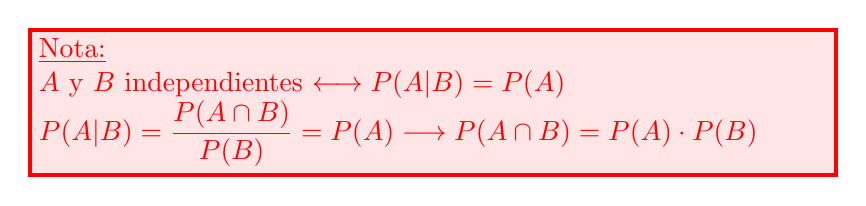
\begin{tikzpicture}
	\node[red, draw=red, fill=red!10, line width=1.5, text width=10cm] {\underline{Nota:}\\
	$A$ y $B$ independientes $\longleftrightarrow P(A|B)=P(A)$\\
	$P(A|B)=\dfrac{P(A\cap B)}{P(B)}=P(A)\longrightarrow P(A\cap B)=P(A)\cdot P(B)$
	};
\end{tikzpicture}
\subsection{Distribuciones condicionadas}
\subsubsection{Caso continuo}

\begin{itemize}[label=\color{red}\textbullet, leftmargin=*]
	\item \color{lightblue}Distribución condicionada al valor de una variable
\end{itemize}

Sea $X=(X_1,\dots,X_k)$ un vector aleatorio continuo con función de densidad $f$.\\
Sea $X_i$ una componente arbitraria y $x_i^*\in\R$ tal que $f_{X_i}(x_i^*)>0$.\\
Se define la \lb{distribución condicionada} de $(X_1,\dots,X_{i-1},X_{i+1},\dots,X_k)$ a $(X_i=x_i^*)$ como la determinada por la función de densidad:

\[ f_{X_1,\dots,X_{i-1},\dots,X_k|X_i=x_i^*}(x_1,\dots,x_{i-1},x_{i+1},\dots,x_k|x_i^*)=\dfrac{f(x_1,\dots,x^*,\dots,x_k)}{f_{X_i}(x_i^*)}. \]


\begin{itemize}[label=\color{red}\textbullet, leftmargin=*]
	\item \color{lightblue}Distribución condicionada a valores de varias variables
\end{itemize}
Sea $X=(X_1,\dots,X_k)$ un vector aleatorio continuo con función de densidad $f$.\\
Sea $(X_{i_1},\dots,X_{i_m})$ un subvector arbitrario y $(x_{i_1}^{*},\dots,x_{i_m}^*)\in\R^m$ tal que: \[ f_{X_{i_1},\dots,X_{i_m}}(x_{i_1}^*,\dots,x_{i_m}^*)>0. \]
Se define la \lb{distribución condicionada} de $(X_1,\dots,X_{i_{1}-1},X_{i_1+1},\dots,X_{i_m-1};X_{i_m+1},\dots,X_k)$ a $(X_{i_1}=x_{i_1}^*,\dots,X_{i_m}=x_{i_m^*})$ como la determinada por la función de densidad:
\[ f_{X_1,\dots,X_{i_{1}-1},X_{i_1+1},\dots,X_{i_m-1},\dots,X_k|X_{i_1}=x_{i_1}^*,\dots,X_{i_m}=x_{i_m^*}}(x_1,\dots,x_{i-1},x_{i+1},\dots,x_{i_m-1},x_{i_m+1},\dots,x_k|x_i^*)=\dfrac{f(x_1,\dots,x_{i_1}^*,\dots,x_{i_m}^*\dots,x_k)}{f_{X_{i_1},\dots,X_{i_m}}(x_{i_1}^*,\dots,x_{i_m}^*)} \]
\subsubsection{Caso discreto}
\begin{itemize}[label=\color{red}\textbullet, leftmargin=*]
	\item \color{lightblue}Distribución condicionada al valor de una variable
\end{itemize}
Sea $X=(X_1,\dots,X_k)$ un vector aleatorio discreto.\\
Sea $X_i$ una componente arbitraria y $x_i^*\in\R$ tal que \[ P[X_i=x_i^*]>0. \]
Se define la \lb{distribución condicionada} de $(X_1,\dots,X_{i-1},X_{i+1},\dots,X_k)$ a $(X_i=x_i^*)$ como la determinada por la función masa de probabilidad:

\begin{center}
$P[X_1=x_1,\dots,X_{i-1}=x_{i-1},X_{i+1}=x_{i+1},\dots,X_k=x_k|X_i=x_i^*]=\dfrac{P[X_1=x_1,\dots,X_{i-1}=x_{i-1},X_i=x_i^*,X_{i+1}=x_{i+1},\dots,X_k=x_k]}{P[X_i=x_i^*]} $
\end{center}

para todo $(x_1,\dots,x_{i-1},x_{i+1},\dots,x_k)$ tal que $x_1,\dots,x_{i-1},x_i^*,x_{i+1},\dots,x_k\in\mathcal{S}$.

\begin{itemize}[label=\color{red}\textbullet, leftmargin=*]
	\item \color{lightblue}Distribución condicionada a valores de varias variables
\end{itemize}
Sea $X=(X_1,\dots,X_k)$ un vector aleatorio discreto.

Sea $X_{i_1},\dots,X_{i_m}$ un subvector arbitrario y $(x_{i_1}^*,\dots,x_{i_m}^*)\in\R^m$ tal que \[ P[X_{i_1}=x_{i_1}^*,\dots,X_{i_m}=x_{i_m}^*]>0. \]
Se define la \lb{distribución condicionada} de $(X_1,\dots,X_{i_1-1},X_{i_1+1},\dots,X_{i_m-1},X_{i_m+1},\dots,X_k)$ a $(X_{i_1}=x_{i_1}^*,\dots,X_{i_m}=x_{i_m}^*)$ como la determinada por la función masa de probabilidad:

\begin{center}
$P[X_1=x_1,\dots,X_{i_{1}-1}=x_{i_1-1},X_{i_1+1}=x_{i_1+1},\dots,X_{i_m-1}=x_{i_m-1},X_{i_m+1}=x_{i_m+1},\dots,X_k=x_k|X_{i_1}=x_{i_1}^*,\dots,X_{i_m}=x_{i_m^*}]=\dfrac{P[X_1=x_1,\dots,X_{i_1}=x_{i_1}^*,\dots,X_{i_m}=x_{i_m}^*,\dots,X_k=x_k]}{P[X_{i_1}=x_{i_1}^*,\dots,X_{i_m}=x_{i_m}^*]}$
\end{center}
para todo $(x_1,\dots,x_{i_1},x_{i_1+1},\dots,x_{i_m-1},x_{i_m+1},\dots,x_k)$, tal que $(x_1,\dots,x_{i_1}^*,\dots,x_{i_m}^*,\dots,x_k)\in\mathcal{S}$

\subsection{Distribución normal multivariante $\mathcal{N}_k(\mu,V)$}
\begin{enumerate}[label=\arabic*)]
	\item Función de densidad
\end{enumerate}
\[ f(x)=\dfrac{1}{\sqrt{|V|(2\pi)^k}}\exp\left(-\dfrac{1}{2}(x-\mu)'V^{-1}(x-\mu)\right), \]para $x\in\R^k$, donde $\mu$ es un vector $k$-dimensional y $V$ es una matriz $k\times k$ simétrica y definida positiva.

\begin{itemize}[label=\color{red}\textbullet, leftmargin=*]
	\item \color{lightblue}Definiciones
\end{itemize}
Una matriz simétrica $A$, de dimensión $k\times k$, se dice que es \lb{definida positiva} si se verifica que $x'Ax>0$ para cualquier vector no nulo $x\in\R^k$.

Una matriz simétrica $A$, de dimensión $k\times k$, se dice que es \lb{semidefinida positiva} si se verifica que $x'Ax\ge0$ para cualquier vector $x\in\R^k$.

¿Cómo calcular la inversa de $V=\begin{pmatrix}
1 & \tfrac{1}{2}\\
\tfrac{1}{2} & 1
\end{pmatrix}$ con \lb{\texttt{R}}?

\vspace{0.5cm}

\begin{lstlisting}
V <- matrix(c(1, 1/2,
						1/2, 1), nrow = 2, ncol = 2, byrow = TRUE)
solve(V)
\end{lstlisting}

\begin{verbatim}
##            [,1]       [,2]
## [1,]  1.3333333 -0.6666667
## [2,] -0.6666667  1.3333333
\end{verbatim}

\subsubsection{Normal bivariante}
\begin{itemize}[label=\color{red}\textbullet, leftmargin=*]
	\item \color{lightblue}Función de densidad
\end{itemize}
Caso bivariante, $k=2$, para $\mu=(0,0)$ y $V=\begin{pmatrix}
1 & \tfrac{1}{2}\\
\tfrac{1}{2} & 1
\end{pmatrix}$.

Cálculo de la función de densidad en $x=(1,1)$ utilizando la función \lb{\texttt{dmvnorm}} de la librería \lb{\texttt{mvtnorm}} de \lb{\texttt{R}}:

\begin{lstlisting}
library("mvtnorm")
V <- matrix(c(1, 1/2,
              1/2, 1), nrow = 2, ncol = 2, byrow = TRUE)
mu <- c(0, 0)
x <- c(1, 1)
dmvnorm(x, mean = mu, sigma = V)
\end{lstlisting}

\begin{verbatim}
## [1] 0.0943539
\end{verbatim}
\begin{itemize}[label=\color{red}\textbullet, leftmargin=*]
	\item \color{lightblue}Función de distribución
\end{itemize}
Cálculo (aproximado) de la función de distribución en $x=(1,1)$ con la función: 

\lb{\texttt{pmvnorm(lower = -Inf, upper = x, mean = mu, sigma = V)}}

\begin{lstlisting}
library("mvtnorm")
V <- matrix(c(1, 1/2,
              1/2, 1), nrow = 2, ncol = 2, byrow = TRUE)
mu <- c(0, 0)
x <- c(1, 1)
pmvnorm(lower = -Inf, upper = x, mean = mu, sigma = V)
\end{lstlisting}

\begin{verbatim}
## [1] 0.7452036
\end{verbatim}

\begin{itemize}[label=\color{red}\textbullet, leftmargin=*]
	\item \color{lightblue}Probabilidad en rectángulos
\end{itemize}
Cálculo (aproximado) de las probabilidades en rectángulos dando los límites inferiores y superiores del rectángulo. Por ejemplo, para calcular \[ P(-1<X_1<1,\:-1<X_2<1) \]
\begin{lstlisting}
library("mvtnorm")
V <- matrix(c(1, 1/2,
              1/2, 1), nrow = 2, ncol = 2, byrow = TRUE)
mu <- c(0, 0)
x1 <- c(- 1, -1)
x2 <- c(1, 1)
pmvnorm(lower = x1, upper = x2, mean = mu, sigma = V)
\end{lstlisting}

\begin{verbatim}
## [1] 0.499718
\end{verbatim}

Su representación gráfica:

\begin{lstlisting}
f <- function(x1, x2) dmvnorm(data.frame(x1, x2), mu, V)
x <- seq(-3, 3, length = 50)
y <- seq(-3, 3, length = 50)
z <- outer(x, y, f)
persp(x, y, z, xlab = 'x1', ylab = 'x2', zlab = 'f(x1, x2)', col = 'orange', main = "Función de densidad")
\end{lstlisting}

\begin{center}
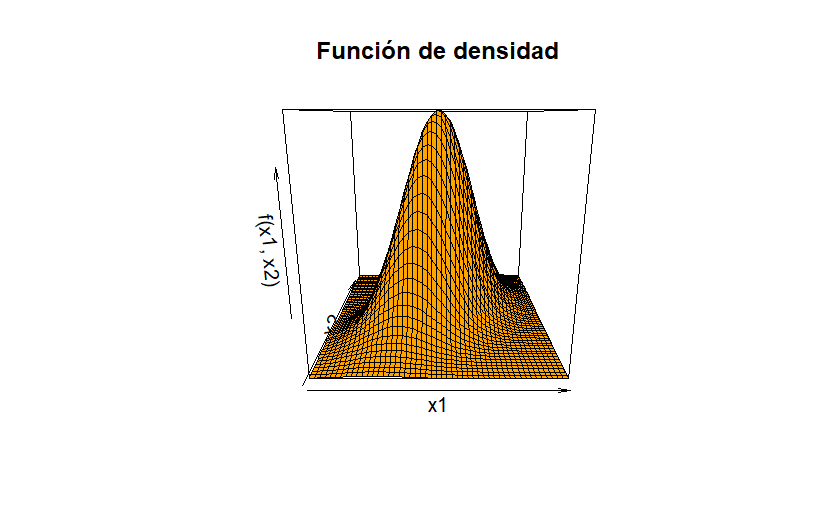
\includegraphics{"Temas/Imágenes/Tema 1/000012.png"}
\end{center}

Su representación gráfica $\left(f(x_1,x_2)=c\right)$ y 50 datos simulados de este modelo

\begin{lstlisting}
#Se fija la semilla para la generación aleatoria
set.seed(123)
#Generación aleatoria del modelo
d <- rmvnorm(50, mu, V)
plot(d, xlab = "X1", ylab = "X2", pch = 20, xlim = c(-3, 3), ylim = c(-3, 3))
contour(x, y, z, nlevels = 4, add = T, col = 'red')
\end{lstlisting}

\begin{center}
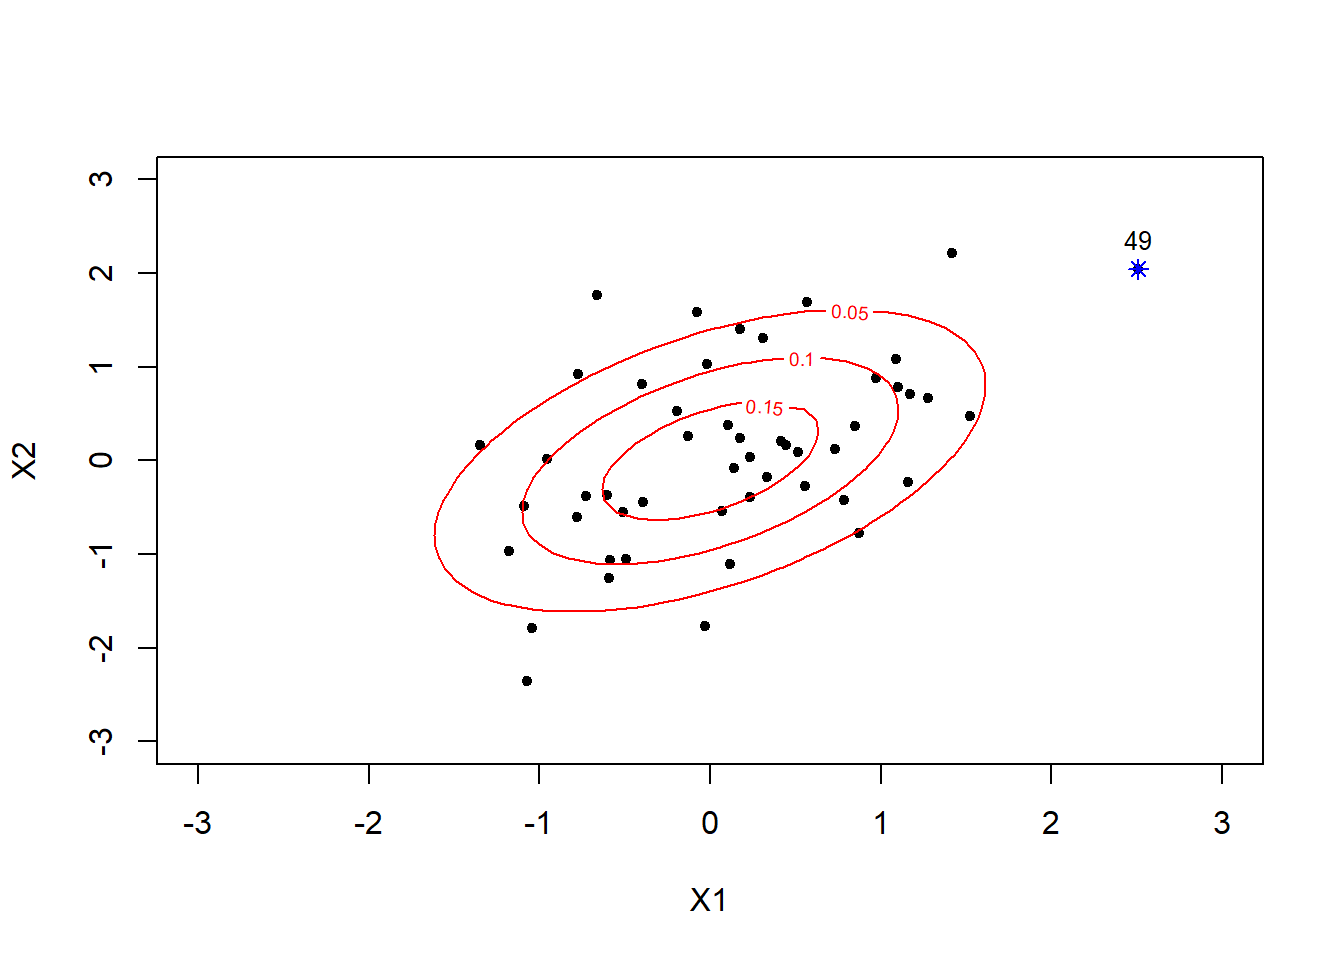
\includegraphics{"Temas/Imágenes/Tema 1/000014.png"}
\end{center}

\begin{itemize}[label=\color{red}\textbullet, leftmargin=*]
	\item \color{lightblue}Distancia de Mahalanobis
\end{itemize}

La distancia de Mahalanobis del vector $x$ al vector $\mu$ basada en la matriz $V$: \[ D=\sqrt{(x-\mu)'V^{-1}(x-\mu)} \]
Tiene en cuenta la diferentes escalas de los datos y sus correlaciones.

Servirá para detectar las observaciones más alejadas del vector de medias que podrían ser observaciones atípicas (\lb{\texttt{outliers}}) que no provengan de nuestra población o contengan errores.
\begin{itemize}[label=$\to$]
\item Cuando se pueda, se deberán chequear y, si es posible, corregir o eliminar.
\item En otros casos, se deberán mantener por ser observaciones correctas que hay que tener en cuenta.
\end{itemize}
\begin{itemize}[label=\color{red}\textbullet, leftmargin=*]
	\item \color{lightblue}Cálculo de la distancia de Mahalanobis
\end{itemize}


Para calcular las distancias de Mahalanobis al cuadrado de los datos al vector de medias (teóricas o muestrales) podemos utilizar la función \lb{\texttt{mahalanobis}}.

\begin{lstlisting}
V <- matrix(c(1, 1/2,
              1/2, 1), nrow = 2, ncol = 2, byrow = TRUE)
mu <- c(0, 0)
dM1 <- mahalanobis(d, mu, V)
dM2 <- mahalanobis(d, colMeans(d), cov(d))
\end{lstlisting}

\begin{itemize}[label=\color{red}\textbullet, leftmargin=*]
	\item \color{lightblue}Distancias de los datos simulados al vector de medias teóricas $\mu$ con respecto a $V$
\end{itemize}

\begin{lstlisting}
summary(dM1)
\end{lstlisting}

\begin{verbatim}
##    Min. 1st Qu.  Median    Mean 3rd Qu.    Max. 
## 0.05216 0.41016 1.26433 1.66615 2.31591 7.13332
\end{verbatim}

\begin{itemize}[label=\color{red}\textbullet, leftmargin=*]
	\item \color{lightblue}¿Dónde se encuentra la observación más alejada del vector de medias?
\end{itemize}

\begin{lstlisting}
d[which.max(dM1), ]
\end{lstlisting}

\begin{verbatim}
## [1] 2.509470 2.046512
\end{verbatim}

\begin{lstlisting}
f <- function(x1, x2) dmvnorm(data.frame(x1, x2), mu, V)
x <- seq(-3, 3, length = 50)
y <- seq(-3, 3, length = 50)
z <- outer(x, y, f)
plot(d, xlab = "X1", ylab = "X2", pch = 20, xlim = c(-3, 3), ylim = c(-3, 3))
points(d[which.max(dM1), 1], d[which.max(dM1), 2], col = "blue", pch = 8)
text(d[which.max(dM1), 1], d[which.max(dM1), 2], which.max(dM1), cex = 0.8, pos = 3)
contour(x, y, z, nlevels = 4, add = T, col = 'red')
\end{lstlisting}

\begin{center}
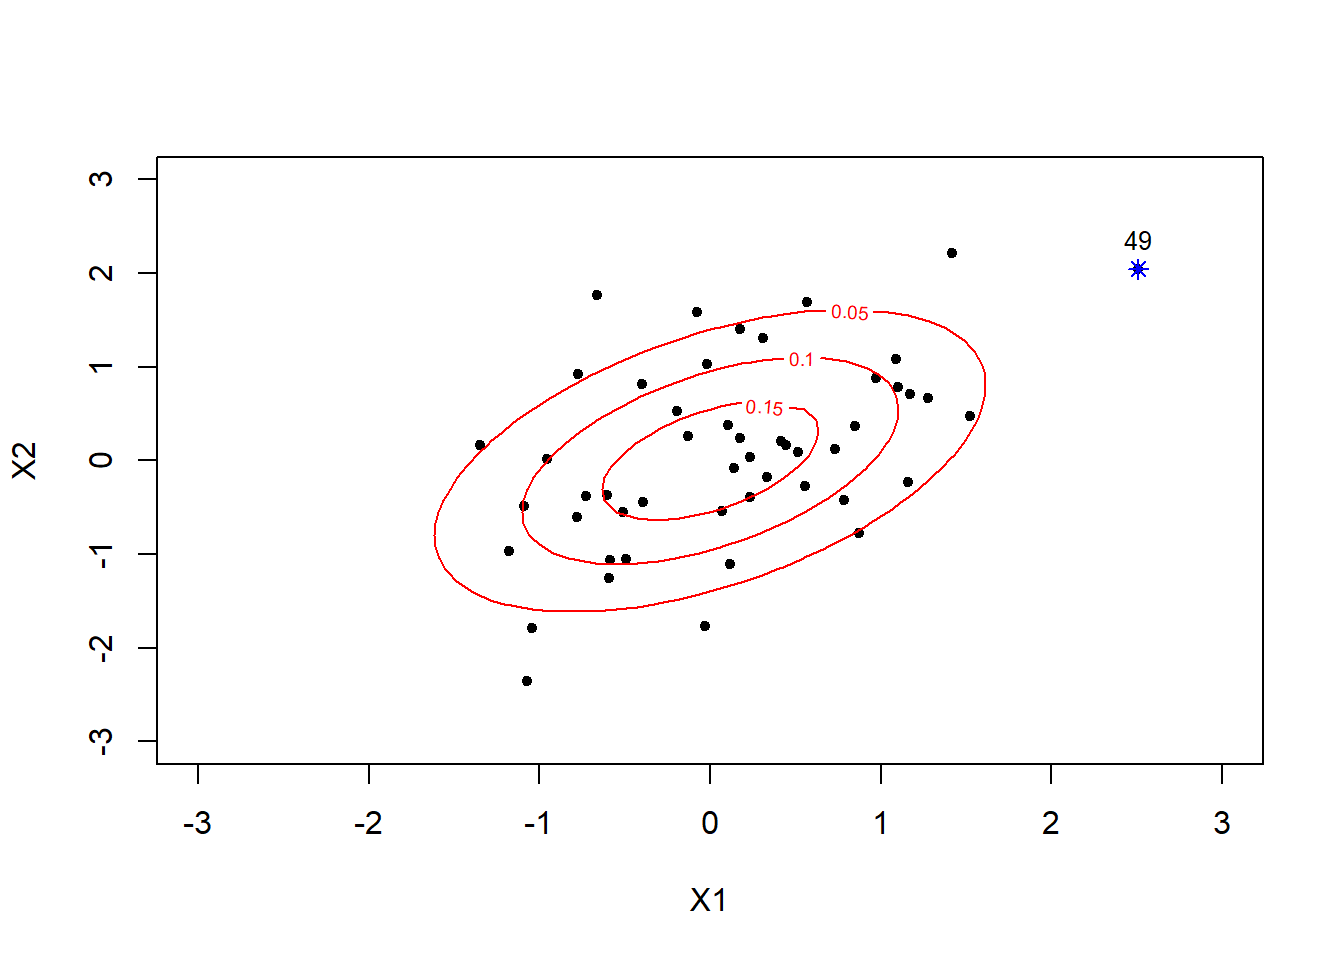
\includegraphics{"Temas/Imágenes/Tema 1/000014.png"}
\end{center}
\begin{itemize}[label=\color{red}\textbullet, leftmargin=*]
	\item \color{lightblue}Distancias de los datos simulados al vector de medias muestrales $\overline{x}$ con respecto a $\mathcal{S}$
\end{itemize}
\begin{lstlisting}
summary(dM2)
\end{lstlisting}

\begin{verbatim}
##    Min. 1st Qu.  Median    Mean 3rd Qu.    Max. 
## 0.02114 0.67111 1.52636 1.96000 2.64131 8.65906
\end{verbatim}

\begin{itemize}[label=\color{red}\textbullet, leftmargin=*]
	\item \color{lightblue}¿Dónde se encuentra la observación más alejada del vector de medias?
\end{itemize}

\begin{lstlisting}
d[which.max(dM2), ]
\end{lstlisting}

\begin{verbatim}
## [1] 2.509470 2.046512
\end{verbatim}

\begin{lstlisting}
f <- function(x1, x2) dmvnorm(data.frame(x1, x2), colMeans(d), cov(d))
x <- seq(-3, 3, length = 50)
y <- seq(-3, 3, length = 50)
z <- outer(x, y, f)
plot(d, xlab = "X1", ylab = "X2", pch = 20, xlim = c(-3, 3), ylim = c(-3, 3))
points(d[which.max(dM2), 1], d[which.max(dM2), 2], col = "blue", pch = 8)
text(d[which.max(dM2), 1], d[which.max(dM2), 2], which.max(dM2), cex = 0.8, pos = 3)
contour(x, y, z, nlevels = 4, add = T, col = 'magenta')
\end{lstlisting}

\begin{center}
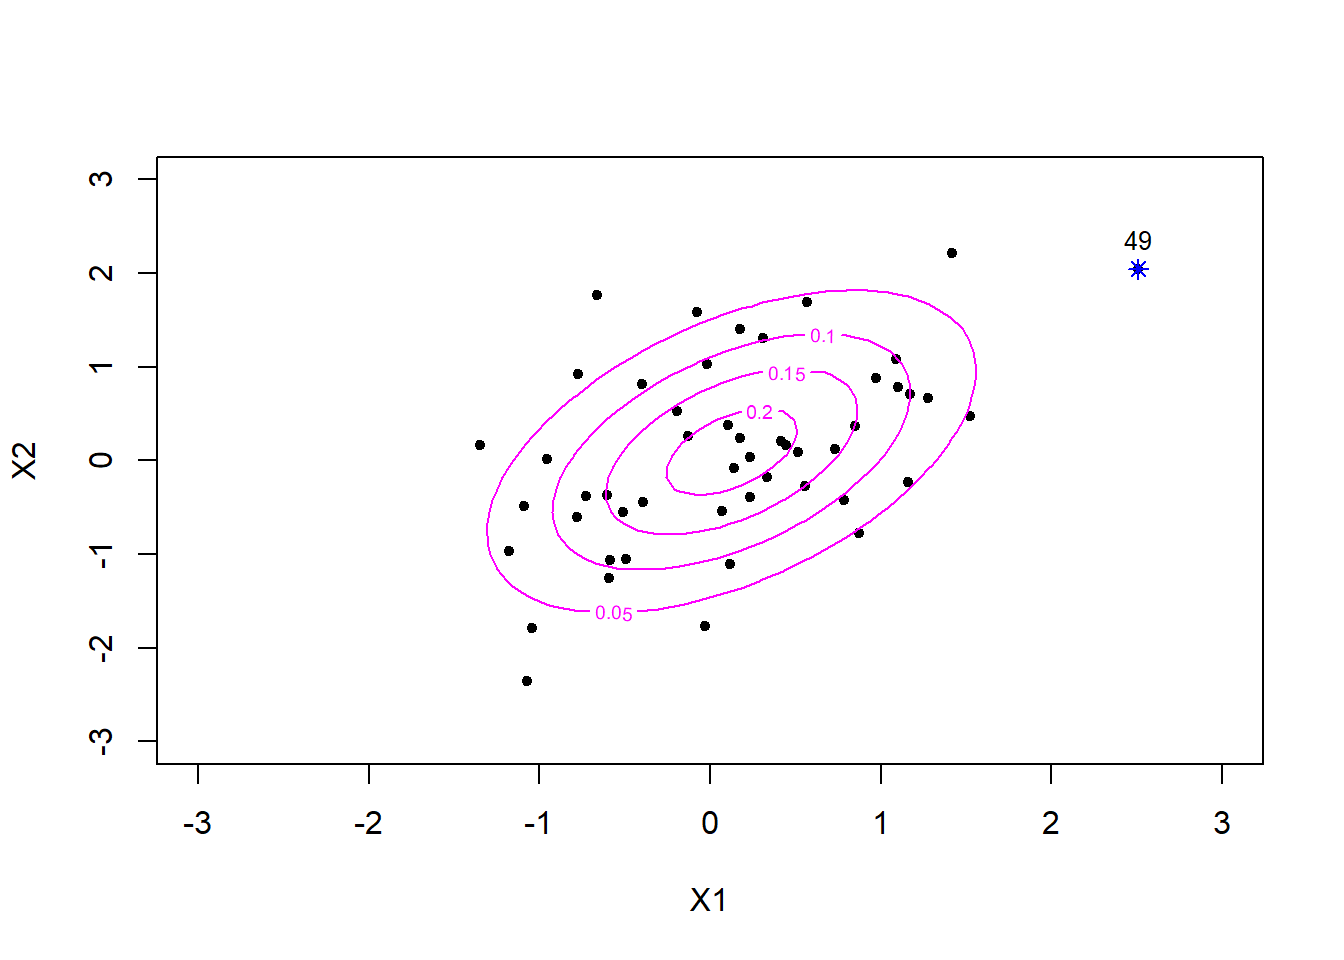
\includegraphics{"Temas/Imágenes/Tema 1/000015.png"}
\end{center}
\subsection{Distribución multinomial $\mathcal{M}_k(n,p_1,\dots,p_k)$}
\begin{itemize}[label=\color{red}\textbullet, leftmargin=*]
	\item \color{lightblue}Modelo multinomial
\end{itemize}
$(X_1,\dots,X_k)$: variables aleatorias que representan el número de veces que ocurre el suceso $A_i$ en un experimento aleatorio repetido $n$ veces con $k$ opciones dadas por $\{A_1,\dots,A_k\}$ y con probabilidades constantes $p_i=P(A_i)$, para $i=1,\dots,k$.
\lb{Función masa de probabilidad conjunta:} \[ p(x_1,\dots,x_k)=P[X_1=x_1,\dots,X_k=x_k]=\dfrac{n!}{x_1!\cdots x_k!}p_1^{x_1}\cdots p_k^{x_k}, \] para enteros no negativos tales que $x_1+\cdots+x_k=n$ y donde $p_i\in[0,1]$ satisface $p_1+\cdots+p_k=1$.

\lb{Distribuciones marginales:} $X_i$ sigue una distribución binomial $B(n,p_i)$, con $E(X_i)=np_i$.
\subsection{Estadístico de Pearson}
\begin{itemize}[label=\color{red}\textbullet, leftmargin=*]
	\item \color{lightblue}Discrepancias entre lo observado y lo esperado
\end{itemize}
\lb{Contexto:} Lanzamos un dado $n=$ veces, $p_i=\frac{1}{6}$ para todo $i$, y los valores esperados son $np_i=10$, para $i=1,\dots,6$.

\lb{Objetivo:} Medir las discrepancias entre valores observados y esperados.

Sea $X=(X_1,\dots,X_k)$ una \va con distribución multinomial, entonces el estadístico \[ T=\sum_{i=1}^{k}\dfrac{X_i-np_i}{np_i} \]sigue una distribución Chi-cuadrado $\chi_{k-1}^2$ de Pearson con $k-1$ grados de libertad, cuando $n\longrightarrow\infty$.
\subsection{Medias y covarianzas}
\begin{itemize}[label=\color{red}\textbullet, leftmargin=*]
	\item \color{lightblue}Definiciones
\end{itemize}
Dado el vector aleatorio.
\begin{itemize}[label=$\to$]
\item El \lb{vector de medias} (o \lb{esperanza matemática} de $X$) se define como: \[ \mu\coloneq E[X]=(E[X_1],\dots,E[X_k])'=(\mu_1,\dots,\mu_k)' \](note que es un vector columna).
\item La \lb{matriz de covarianzas (o varianzas-covarianzas)} se define como: \[ V=(\sigma_{i,j}), \] donde $\sigma_{i,j}$ es la covarianza entre $X_i$ y $X_j$, definida como: \[ \sigma_{i,j}=\cov(X_i,X_j)=E\left[(X_i-\mu_i)(X_j-\mu_j)\right]=E[X_iX_j]-\mu_i\mu_j \]Notemos que $\sigma_{i,i}=E\left[(X_i-\mu_i)^2\right]=\var(X_i)=\sigma_i^2$.
\end{itemize}
\begin{itemize}[label=\color{red}\textbullet, leftmargin=*]
	\item \color{lightblue}Cálculo de la esperanza matemática
\end{itemize}
La media de cada componente $X_i$ del vector puede calcularse a partir de la distribución conjunta o a partir de la marginal.
\begin{itemize}[label=\color{lightblue}$\to$]
\item \lb{Caso discreto:} \[ \begin{aligned}
E[X_i]&=\sum_{x_i}x_i P[X_i=x_i]\\
&=\sum_{x_1,\dots,x_k}x_i P[X_1=x_1,\dots,X_k=x_k]
\end{aligned} \]
\item \lb{Caso continuo:} \[ \begin{aligned}
E[X_i] &=\int_{\R }x_if_{X_i}(x_i)\dx_i\\
&=\int_{\R^k}x_if(x_1,\dots,x_k)\dx_1\cdots\dx_k
\end{aligned} \]
\end{itemize}

\subsubsection{Esperanza de la transformación $g:\R^k\longrightarrow\R$}
\begin{itemize}[label=\color{red}\textbullet, leftmargin=*]
	\item \color{lightblue}Caso discreto
\end{itemize}
Sea $g:\R^k\longrightarrow\R$ una función medible $\longrightarrow Y=g(X)$ es una \va. 

Si $X$ es de tipo discreto, \[ \exists E[g(X)]\longleftrightarrow\sum_{x_1,\dots,x_k}\left|g(x_1,\dots,x_k)\right|P[X_1=x_1,\dots,X_k=x_k]<\infty \]
Y en caso de existir: \[ E[g(X_1,\dots,X_k)]=\sum_{x_1,\dots,x_k}g(x_1,\dots,x_k)P[X_1=x_1,\dots,X_k=x_k] \]
\begin{itemize}[label=\color{red}\textbullet, leftmargin=*]
	\item \color{lightblue}Caso continuo
\end{itemize}
Sea $g:\R^k\longrightarrow\R$ una función medible $\longrightarrow Y=g(X)$ es una \va.

Si $X$ es de tipo continuo, \[ \exists E[g(X)]\longleftrightarrow\int_{\R^k}\left|g(x_1,\dots,x_k)\right|f_X(x_1,\dots,x_k)\dx_1\cdots\dx_k<\infty \]
Y en caso de existir: \[ E[g(X_1,\dots,X_k)]=\int_{\R^k}g(x_1,\dots,x_k)f_X(x_1,\dots,x_k)\dx_1\cdots\dx_k. \]
\begin{itemize}[label=\color{red}\textbullet, leftmargin=*]
	\item \color{lightblue}Propiedades
\end{itemize}
$V$ es una matriz \lb{simétrica} y \lb{semidefinida positiva} ($x'Vx\ge0$, para todo $x\in\R^k$).

En forma matricial, \[ V=E\left[(X-\mu)(X-\mu)'\right]=E[XX']-\mu\mu'.\] donde la \lb{esperanza de una matriz aleatoria} se define como la matriz de las esperanzas de cada variable.

Si $X_i$ y $X_j$ son \lb{independientes}, entonces \[ E[X_iX_j]=E[X_i]E[X_j] \]y, por lo tanto, $\cov(X_i,X_j)=0$. El recíproco no es cierto.

Si $X\longrightarrow\mathcal{N}_k(\mu, V)$, se puede demostrar que $\mu$ es el vector de medias y $V$ es la matriz de covarianzas.
\subsection{Correlación}
La \lb{correlación (lineal de Pearson)} entre $X_i$ y $X_j$ se define como \[ \rho_{i,j}=\corr(X_i,X_j)=\dfrac{\sigma_{i,j}}{\sigma_i\sigma_j} \]siendo $\rho_{i,i}=\corr(X_i,X_j)=1$.

Mide el \lb{grado de relación lineal} entre $X_i$ y $X_j$.

Puede demostrarse que \[ -1\le\rho_{i,j}\le1. \]
Se dice que $X_i$ y $X_j$ son \lb{incorreladas} si $\rho_{i,j}=0$.

Si son independientes serán incorreladas, pero el recíproco no es cierto.

La \lb{matriz de correlaciones} es $R=(\rho_{i,j})$.
\subsection{Correlación entre vectores aleatorios}
Análogamente, si $X$ e $Y$ son \veas (de dimensiones cualesquiera), se define su \lb{matriz de covarianzas} como \[ \cov(X,Y)=(\cov(X_i,Y_j)) \] y su \lb{matriz de correlaciones} como \[ \corr(X,Y)=(\corr(X_i,Y_j)). \]Puede demostrarse que \[ \cov(X,Y)=E[(X-E[X])(Y-E[Y])']. \]Evidentemente, $\cov(X)=\cov(X,X)$.
\begin{itemize}[label=\color{red}\textbullet, leftmargin=*]
	\item \color{lightblue}Propiedades
\end{itemize}
Si $X,Y,Z$ son vectores (columna) aleatorios, se verifican las propiedades siguientes:
\begin{enumerate}[label=\color{lightblue}\arabic*)]
	\item $E[a_1g_1(X)+a_2g_2(X)]=a_1E[g_1(X)]+a_2E[X_2]$, donde $a_1,a_2\in\R$ y $g_1$ y $g_2$ son funciones medible de vectores aleatorios.
	\item $X=(Y,Z),E_X[g(Y)]=E_Y[g(Y)]$, donde $g$ es una función medible de un vector aleatorio, $E_X$ denota la esperanza en la distribución conjunta y $E_Y$ en la distribución marginal.
	\item Si $X$ e $Y$ son independientes, entonces \[ E[g_1(X)g_2(Y)]=E[g_1(X)]E[g_2(Y)], \] donde $g_1$ y $g_2$ son funciones medibles cualesquiera de \veas.
	\item $E[AX+b]=AE[X]+b,A\in M_{m,k}b'\in\R^m$.
	\item $\cov(X_i,X_j)=E[X_iX_j]-E[X_i]E[X_j]$.
	\item Si $X_1,\dots,X_k$ son independientes, $\cov(X_i,X_j)=0$.
	\item $\var(X_i+X_j)=\var(X_i)+2\cov(X_i,X_j)+\var(X_j)$.
	\item $\cov(aX_i+b,cX_j+d)=ac\cov(X_i,X_j)$, donde $a,b,c,d\in\R$.
	\item $\cov(X)=E[(X-\mu)(X-\mu)']=E[XX']-\mu\mu'$.
	\item $\var(a'X)=a'\cov(X)a=\sum_{i,j}a_ia_j\sigma_{i,j}$, donde $a\in\R^k$.
	\item $\cov(AX+b)=A\cov(X)A'$, donde $A\in M_{m,k}$ y $b'\in\R^m$.
	\item Si $X_1,\dots,X_k$ son independientes, $\corr(X_i,X_j)=0$.
	\item $\corr(aX_i+b,cX_j+d)=\corr(X_i,X_j)$, donde $a,b,c,d\in\R$.
	\item $-1\le\corr(X_i,X_j)\le1$.
	\item $\corr(X_i,aX_i+b)=\pm1$, donde $a,b\in\R$ (según el signo de $a$).
	\item $\corr(X)=\delta^{-1}\cov(X)\delta^{-1}$, donde $\delta$ es la matriz diagonal formada por las desviaciones típicas $\left(\delta=\mathrm{diag}(\sigma_1,\dots,\sigma_k)\right)$.
	\item $\cov(X,Y)=\left(\cov(X_i,Y_j)\right)=\cov(Y,X)'$.
	\item $\cov(X+Z,Y)=\cov(X,Y)+\cov(Z,Y)$
	\item Si $X$ e $Y$ tienen la misma dimensión, entonces $\cov(X+Y)=\cov(X)+\cov(X,Y)+\cov(Y,X)+\cov(Y)$.
	\item $\cov(AX,BY)=A\cov(X,Y)B'$, donde $A$ y $B$ son matrices (de dimensiones adecuadas).
	\item Si $X$ e $Y$ independientes, entonces $\cov(X,Y)=0$.
\end{enumerate}
\begin{itemize}[label=\color{red}\textbullet, leftmargin=*]
	\item \color{lightblue}Demostración apartado (10)
\end{itemize}
Directamente se tiene que: \[ \var(a'X)=\cov(a'X,a'X)=E[a'(X-\mu)(X-\mu)'a]=a\cov(X)a \]
Como consecuencia, se obtiene que la matriz de covarianzas $\cov(X)$ es semidefinida positiva ya que $\var(a'X)\ge0$.

Lo mismo le ocurre a la matriz de correlaciones $\corr(X)$ ya que es la matriz de covarianzas de las \vas tipificadas $Z_i=\dfrac{X_i-\mu_i}{\sigma_i}$.
\subsection{Resultados básicos de la inferencia}
\begin{itemize}[label=\color{red}\textbullet, leftmargin=*]
	\item \color{lightblue}Contexto
\end{itemize}
En la práctica, todas las medidas, varianzas y covarianzas serán desconocidas por lo que tenemos que estimarlas.\\
Para ello dispondremos de una muestra de individuos (objetos) en los que se han medido todas las variables.\\
Proporcionamos resultados básicos de inferencia para poder aplicar las técnicas multivariantes que desarrollaremos en temas posteriores.\\
Se ilustran estos procedimientos de inferencia con conjuntos de datos de \lb{\texttt{R}}, accesibles con \lb{\texttt{data()}}.
\subsubsection{¿Cómo se representan las muestras aleatorias?}

\begin{wrapfigure}[5]{r}{0.4\textwidth}
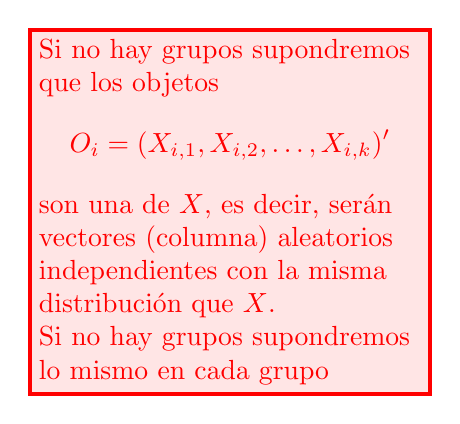
\begin{tikzpicture}
	\node[red, draw=red, fill=red!10, line width=1.5, text width=0.4\textwidth] {Si no hay grupos supondremos que los objetos \[ O_i=(X_{i,1},X_{i,2},\dots,X_{i,k})' \] son una \mas de $X$, es decir, serán vectores (columna) aleatorios independientes con la misma distribución que $X$.\\
	Si no hay grupos supondremos lo mismo en cada grupo
	};
\end{tikzpicture}
\end{wrapfigure}

\begin{itemize}[label=\color{red}\textbullet, leftmargin=*]
	\item \color{lightblue}Matriz de la \mas
\end{itemize}

En general, nuestra muestra aleatoria se representará como:
\[ \begin{array}{cccccc}
i & X_1 & X_2 & \cdots & X_k & Y \\ \hline
O_1 & X_{1,1} & X_{1,2} & \cdots & X_{1,k} & Y_1 \\
\cdots & \cdots & \cdots & \cdots & \cdots & \cdots \\
O_i & X_{i,1} & X_{i,2} & \cdots & X_{i,k} & Y_i \\
\cdots & \cdots & \cdots & \cdots & \cdots & \cdots \\
O_n & X_{n,1} & X_{n,2} & \cdots & X_{n,k} & Y_n \\ \hline
\end{array} \]
La variable $Y$ solo se usará para detonar la variable respuesta en regresión.

En algunos casos usaremos la matriz $M=(X_{i,j})$ que será una matriz aleatoria.
\subsubsection{¿Cómo se muestran los valores muestrales?}

\begin{wrapfigure}{r}{0.4\textwidth}
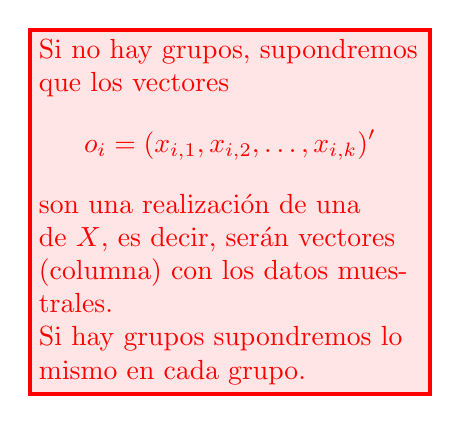
\begin{tikzpicture}
	\node[red, draw=red, fill=red!10, line width=1.5, text width=0.4\textwidth] {Si no hay grupos, supondremos que los vectores \[ o_i=(x_{i,1},x_{i,2},\dots,x_{i,k})' \] son una realización de una \mas de $X$, es decir, serán vectores (columna) con los datos muestrales.\\
	Si hay grupos supondremos lo mismo en cada grupo.
	};
\end{tikzpicture}
\end{wrapfigure}

\begin{itemize}[label=\color{red}\textbullet, leftmargin=*]
	\item \color{lightblue}Matriz de datos
\end{itemize}

En general, nuestra muestra se representará como: 
\[ \begin{array}{cccccc}
i & x_1 & x_2 & \cdots & x_k & y \\ \hline
o_1 & x_{1,1} & x_{1,2} & \cdots & x_{1,k} & y_1 \\
\cdots & \cdots & \cdots & \cdots & \cdots & \cdots \\
o_i & x_{i,1} & x_{i,2} & \cdots & x_{i,k} & y_i \\
\cdots & \cdots & \cdots & \cdots & \cdots & \cdots \\
o_n & x_{n,1} & x_{n,2} & \cdots & x_{n,k} & y_n \\ \hline
\end{array} \]
La variable $Y$ solo se usará para detonar la variable respuesta en regresión.

En algunos casos usaremos la matriz de datos $M=(x_{i,j})$

\subsubsection{El conjunto de datos \textbf{\texttt{LifeCycleSavings}}}

\begin{itemize}[label=\color{red}\textbullet, leftmargin=*]
	\item \color{lightblue}Cargamos los datos y visualizamos las primeras filas
\end{itemize}

\begin{lstlisting}
datos <- LifeCycleSavings
head(datos, n = 6)
\end{lstlisting}

\begin{verbatim}
##              sr pop15 pop75     dpi ddpi
## Australia 11.43 29.35  2.87 2329.68 2.87
## Austria   12.07 23.32  4.41 1507.99 3.93
## Belgium   13.17 23.80  4.43 2108.47 3.82
## Bolivia    5.75 41.89  1.67  189.13 0.22
## Brazil    12.88 42.19  0.83  728.47 4.56
## Canada     8.79 31.72  2.85 2982.88 2.43
\end{verbatim}

\begin{itemize}[label=\color{red}\textbullet, leftmargin=*]
	\item \color{lightblue}¿Qué información está recogida en el conjunto de datos?
\end{itemize}
Con la instrucción \lb{\texttt{help(LifeCycleSavings)}} conocemos qué información está contenida en el conjunto:
\begin{itemize}
\item \lb{\texttt{sr}:} incremento de los ahorros personales 1960-1970.
\item \lb{\texttt{pop15}:} \% población menor de 15 años.
\item \lb{\texttt{pop75}:} \% población menor de 75.
\item \lb{\texttt{dpi}:} ingresos per-capita.
\end{itemize}
\subsection{Estimador para el vector de medias $\mu$}
Vector de \lb{medias muestrales}, también llamado \lb{objeto medio}, se define como: \[ \overline{O}=\overline{X}=\left(\overline{X}_1,\dots,\overline{X}_k\right)'=\dfrac{1}{n}\sum_{i=1}^{n}O_i, \] donde $ \overline{X}_j=\dfrac{1}{n}\sum_{i=1}^{n}X_{i,j}$.

Se puede demostrar fácilmente que:
\begin{itemize}[label=$\to$]
\item $E(\overline{O})=\mu$ (estimador centrado de $\mu$)
\item $\cov(\overline{O})=\dfrac{V}{n}$
\end{itemize}
\subsubsection{¿Dónde se encuentra el vector de medias muestrales?}
\begin{itemize}[label=\color{red}\textbullet, leftmargin=*]
	\item \color{lightblue}Propiedad
\end{itemize}
$\overline{O}$ es el punto de $\R^k$ que minimiza la suma de las distancias al cuadrado (\lb{error cuadrático medio}, MSE), es decir, es la solución de \[ \underset{P\in\R^k}{\min}MSE=\sum_{i=}^{n}d^2(O_i,P), \] donde $d$ representa la distancia Euclídea, definida para dos vectores $x,y\in\R^k$ como \[ d(x,y)=\sqrt{\sum_{j=1}^{k}(x_j-y_j)^2}. \]
\subsection{Estimador para la matriz de covarianzas $V$}

Para estimar $\sigma_{i,j}$ usaremos
\begin{itemize}[label=$\to$]
\item La \lb{covarianza muestral:} $\hat{\sigma}_{i,j}=\dfrac{1}{n}\sum_{l=1}^{n}(X_{l,i}-\overline{X}_i)(X_{l,j}-\overline{X}_j)$
\item La \lb{cuasi-covarianza muestral:} \[ \mathcal{S}_{i,j}=\dfrac{1}{n-1}\sum_{l=1}^{n}(X_{l,i}-\overline{X}_i)(X_{l,j}-\overline{X}_j) \]
\end{itemize}
Para estimar $V$ usaremos:
\begin{itemize}[label=$\to$]
\item $\hat{V}=(\hat{\sigma}_{i,j})=\dfrac{1}{n}\sum_{l=1}^{n}(O_l-\overline{O})(O_l-\overline{O})'$
\item $\mathcal{S}=(\mathcal{S}_{i,j})=\dfrac{1}{n-1}\sum_{n-1}^{n}(O_l-\overline{O})(O_l-\overline{O})'$
\end{itemize}
Se verifica que $E(\mathcal{S})=V$ (estimador centrado de $V$).

\subsubsection{Para una distribución normal}
\begin{itemize}[label=\color{red}\textbullet, leftmargin=*]
	\item \color{lightblue}Proposición
\end{itemize}
Si $X\longrightarrow\mathcal{N}_k(\mu,V)$ entonces se verifica que: 
\begin{itemize}
\item $\overline{O}\longrightarrow\mathcal{N}_k\left(\mu,\tfrac{V}{n}\right)$
\item $\overline{O}$ y $\hat{V}$ son los \lb{estimadores máximos verosímiles} de $\mu$ y $V$, respectivamente.
\item Además, $\overline{O}$ y $\hat{V}$ son \lb{independientes entre sí}. Por tanto, también $\overline{O}$ y $\mathcal{S}$ son independientes entre sí.
\item La distribución aleatoria \[ n\hat{V}=(n-1)\mathcal{S} \]se conoce como \lb{distribuidor de Wishart}.
\end{itemize}
\begin{itemize}[label=\color{red}\textbullet, leftmargin=*]
	\item \color{lightblue}Test de normalidad multivariante: Test de Shapiro-Wilk
\end{itemize}
Para la aplicación de algunas técnicas multivariantes la hipótesis de normalidad es importante y debe ser contrastada. \[ \begin{array}{l}
H_0:(X_1,\dots,X_k)\rightarrow\mathcal{N}_k(\mu,V)\\
H_1:(X_1,\dots,X_k)\nrightarrow\mathcal{N}_k(\mu,V)\\
\end{array} \]
Podremos utilizar la función \lb{\texttt{mshapiro.test}} de la librería \lb{\texttt{mvnormtest}} de \lb{\texttt{R}} para realizar el test de normalidad multivariante de Shapiro-Wilk.
\begin{itemize}[label=$\to$]
\item Si aplicamos el test a los 50 datos simulados de la normal bivariante lógicamente obtnedremos un $p$-valor que apoya la hipótesis nula.
\end{itemize}

\begin{lstlisting}
library("mvnormtest")
V <- matrix(c(1, 1/2,
              1/2, 1), nrow = 2, ncol = 2, byrow = TRUE)
mu <- c(0, 0)
seed = set.seed(2023)
d <- rmvnorm(50, mu, V)
mshapiro.test(t(d))
\end{lstlisting}

\begin{verbatim}
## [1]  0.6922
\end{verbatim}
\begin{itemize}[label=\color{red}\textbullet, leftmargin=*]
	\item \color{lightblue}Seguimos con \textbf{\texttt{LifeCycleSavings}}
\end{itemize}

Cálculo de las medias muestrales para cada variable.

\begin{lstlisting}
mean(datos$sr); mean(datos$pop15); mean(datos$pop75);  mean(datos$dpi); mean(datos$ddpi)
\end{lstlisting}

\begin{verbatim}
## [1] 9.671
## [1] 35.0896
## [1] 2.293
## [1] 1106.758
## [1] 3.7576
\end{verbatim}

O bien, podemos calcular todas las características de estas variables

\begin{lstlisting}
summary(datos)
\end{lstlisting}

\begin{verbatim}
##        sr             pop15           pop75            dpi         
##  Min.   : 0.600   Min.   :21.44   Min.   :0.560   Min.   :  88.94  
##  1st Qu.: 6.970   1st Qu.:26.21   1st Qu.:1.125   1st Qu.: 288.21  
##  Median :10.510   Median :32.58   Median :2.175   Median : 695.66  
##  Mean   : 9.671   Mean   :35.09   Mean   :2.293   Mean   :1106.76  
##  3rd Qu.:12.617   3rd Qu.:44.06   3rd Qu.:3.325   3rd Qu.:1795.62  
##  Max.   :21.100   Max.   :47.64   Max.   :4.700   Max.   :4001.89  
##       ddpi       
##  Min.   : 0.220  
##  1st Qu.: 2.002  
##  Median : 3.000  
##  Mean   : 3.758  
##  3rd Qu.: 4.478  
##  Max.   :16.710
\end{verbatim}

Cálculo de la matriz de covarianzas muestrales

\begin{lstlisting}
cov(d)
\end{lstlisting}

\begin{verbatim}
##           [,1]      [,2]
## [1,] 1.1101259 0.8347425
## [2,] 0.8347425 1.2075240
\end{verbatim}

Cálculo de la matriz de correlaciones muestrales

En este caso es mejor usar correlaciones muestrales que eliminan el efecto de las unidades: \[ R_{i,j}=\dfrac{\mathcal{S}_{i,j}}{\mathcal{S}_i\mathcal{S}_j}, \] donde $\mathcal{S}_i=\sqrt{\mathcal{S}_{i,i}}$ y $\mathcal{S}_j=\sqrt{\mathcal{S}_{j,j}}$.

Cálculo de la matriz de correlaciones muestrales

\begin{lstlisting}
cor(datos)
\end{lstlisting}

\begin{verbatim}
##               sr       pop15       pop75        dpi        ddpi
## sr     1.0000000 -0.45553809  0.31652112  0.2203589  0.30478716
## pop15 -0.4555381  1.00000000 -0.90847871 -0.7561881 -0.04782569
## pop75  0.3165211 -0.90847871  1.00000000  0.7869995  0.02532138
## dpi    0.2203589 -0.75618810  0.78699951  1.0000000 -0.12948552
## ddpi   0.3047872 -0.04782569  0.02532138 -0.1294855  1.00000000
\end{verbatim}


\begin{tikzpicture}
	\node[red, draw=red, fill=red!10, line width=1.5] {Observamos que algunas variables tienen correlaciones positivas y otras negativas};
\end{tikzpicture}

\newpage

\section{Introducción a los sistemas NoSQL}
\subsection{Introducción a NoSQL}
\textbf{NoSQL} $\longrightarrow$ \textit{hastag} llamativo que se eligió para una conferencia en 2009 (Johan Oskarsson de Last.fm)

Ahora se asocia a cientos de bases de datos diferentes, que se han clasificado en varios tipos (las veremos después), caracterizadas por \textbf{no usar SQL} como modelo de datos.

Más recientemente \textbf{NoSQL $\longrightarrow$ \textit{Not Only SQL}} (no sólo SQL) $\longrightarrow$ Persistencia políglota (\textit{polyglot persistence})

\subsubsection{¿Por qué se plantearon?}
\begin{enumerate}
	\item \textbf{Mayor escalabilidad horizontal}
	\begin{itemize}
		\item conjuntos de datos muy muy grandes
		\item sistemas de alto volumen de escrituras (\textbf{streaming} de eventos, aplicaciones sociales)
	\end{itemize}
	\item \textbf{Demanda de productos de software libre} (crecimiento de las \textit{start-ups})
	\item \textbf{Consultas especializadas} no eficientes en el modelo relacional (JOINs)
	\item \textbf{Expresividad, flexibilidad, dinamismo.} Frustración con \textbf{restricciones} del modelo relacional
\end{enumerate}
\subsubsection{Características}
No se basan en SQL

Modelos de datos más ricos

Orientadas a la \textbf{Escalabilidad}

Generalmente no obligan a definir un esquema
\begin{itemize}
	\item \textbf{Schemaless}
\end{itemize}
Surgidos de la comunidad para solucionar problemas
\begin{itemize}
	\item  muchas \textbf{libres/\emph{open source}}
\end{itemize}
Diseño basado en\textbf{ procesamiento distribuido}

Principios funcionales
\begin{itemize}
	\item \textbf{MapReduce}
\end{itemize}
\subsubsubsection{Categorías de NoSQL}
\begin{itemize}
\item Bases de datos \textit{key-value}\\
\item Bases de datos documentales\\
\item Bases de datos columnares (\textit{wide column})\\
\item Bases de datos de grafos\\
\item Bases de datos de arrays
\end{itemize}
\subsubsection{Evolución desde el modelo relacional}
El \textbf{modelo relacional $\Rightarrow$ predominante en los últimos ˜30 años}\\
Tiene sus raíces en el denominado \textit{business data processing}, procesamiento de
transacciones y \textit{batch}\\
Propuesto por Codd en los 70, \textbf{de alto nivel}\\
Actualmente los \textbf{sistemas SQL están muy optimizados:}
\begin{itemize}
	\item el \textbf{grado de implantación es mayoritario}
\item para el 99 \% de los problemas (que caben en un ordenador) es eficiente y adecuado
\end{itemize}
\subsection{Adopción de NoSQL}
\subsubsection{Análisis}
Dominan los grandes SGBDR\\
El \textit{Open Source} tiene una importancia crucial (PostgreSQL, MySQL, MongoDB, etc.)\\
Varias bases de datos NoSQL entre las 10 primeras. Muchas en las 20 primeras\\
La distancia entre los grandes SGBDR y el primer NoSQL (MongoDB) es de $5\times$\\
Paradigmas más "atrevidos" como el de grafos están entre los 20 primeros (Neo4j)\\
\subsection{Cambio de perspectiva: Red}
\begin{center}
	\includegraphics{"Temas/Tema 2/screenshot001"}
\end{center}
\subsubsubsection{Almacenamiento distribuido}
Desde los 90's: Clústers/NOC/COW: procesamiento masivamente paralelo

Almacenamiento no distribuido

Ahora los nodos $\Rightarrow$ también \textbf{almacenamiento}

Minimizar el verdadero cuello de botella: \textbf{trasiego de información por la red}.

\subsubsubsection{Procesamiento distribuido}
Necesidad de \textbf{paralelización máxima}\\
\textbf{Escalabilidad}\\
Explotar de la \textbf{localidad de los datos}:
\begin{itemize}
	\item Datos producidos se utilizan localmente en siguientes iteraciones
\item Datos recibidos directamente en los \textit{hosts} (clientes simultáneos)
\end{itemize}
Vuelta al modelo funcional inherentemente paralelo: (e.g. \textbf{Map-Reduce})\\
Almacenamiento distribuido: (e.g. \textbf{HDFS})\\
Coordinación distribuida: (e.g. \textbf{Zookeeper})
\subsubsubsection{Modelo de datos}
El modelo relacional limita a tablas con valores primitivos y relaciones \textit{Primary Key/Foreign Key}\\
En programación se utilizan \textbf{listas, arrays, tipos de datos compuestos} (\textit{gap semántico})\\
ACID es \textbf{muy compleja y costosa} en ambientes distribuidos (quizá \textbf{no necesaria} en algunas aplicaciones).

¿Y si se pudiera ver como un \textbf{GRAN ARRAY}?
\begin{itemize}
\item Cada nodo almacenaría una parte del array
\item Búsqueda aleatoria \textbf{muy rápida} (árboles B)
\item Uso de \textbf{filtros de Bloom}
\item Uso de \textbf{objetos complejos} (p. ej. \textbf{documentos JSON}), para mantener la \textbf{localidad espacial de datos relacionados} 
\item Transacciones limitadas al \textbf{objeto complejo}
\end{itemize}
\subsection{Schemaless}
Las Bases de Datos NoSQL (en general) \textbf{no quieren de un esquema}

\textbf{Flexibilidad:} Posibilidad de almacenar entidades con una estructura diferente
\begin{itemize}
	\item Tratar información incompleta.
	\item Evolucionar la base de datos/esquema.
	\item Añadir nuevas características a las aplicaciones
\end{itemize}
\begin{center}
	\includegraphics[width=\linewidth]{"Temas/Tema 2/screenshot002"}
\end{center}
\textbf{Ejemplo:} Añadir el campo \texttt{first_name} a partir del campo \texttt{name}

Los nuevos objetos se crean con el nuevo formato

A la hora de leerlos, se puede hacer:

\begin{lstlisting}[language=c++]
if (user && user.name && !user.first_name) {
	// Docs anteriores a 2013 no tienen first_name
	user.first_name = user.name.split(" ")[0];
}
\end{lstlisting}
En SQL puede ser un proceso muy costoso (procesa toda la tabla, locking, puede que haya que parar las aplicaciones):

\begin{lstlisting}[language=SQL]
ALTER TABLE users ADD COLUMN first_name text;
UPDATE users SET first_name =
	substring_index(name, ' ', 1);
\end{lstlisting}
\subsubsection{¿Cuándo es apropiado \textit{schemaless}?}
\textbf{Objetos heterogéneos}

Estructura de los datos \textbf{impuesta externamente}

Si intuimos que los datos \textbf{cambiarán en el futuro}

\textbf{Sin embargo}

A veces \textbf{un esquema es conveniente}
\begin{itemize}
	\item Facilita el desarrollo y evita inconsistencias
	\begin{itemize}
		\item \texttt{Mongoose} para MongoDB:
	\end{itemize}
	\begin{lstlisting}[language=C++]
var Comment = new Schema({
	name: {type: String, default: 'Anonymous'},
	date: {type: Date, default: Date.now},
	text: Buffer
});
// a setter with on-line modification
Comment.path('name').set(function (v) {
	return capitalize(v);
});
	\end{lstlisting}
\end{itemize}
\subsection{Map-Reduce}
Map-Reduce: origen lenguajes funcionales:
\begin{itemize}
\item \texttt{map()}: Ejecuta una misma función sobre todos los elementos de un conjunto
\item \texttt{reduce()}: Sumariza un conjunto de valores para producir un valor de salida
\end{itemize}
Map-Reduce combina ambas operaciones:
\begin{itemize}
\item Una misma operación \texttt{map()} a cada dato residente en un nodo es realizada de forma paralela en \textbf{todos} los nodos simultáneamente
\item Con los resultados parciales de cada nodo, una función \texttt{reduce()} genera un resultado (o un conjunto de resultados) final
\item Proceso intermedio de \textit{shuffle} para agrupar valores \textbf{con la misma clave} antes del \textbf{reduce()}
\item Resultados parciales en el mismo nodo (localidad) $\Rightarrow$ procesamientos \textbf{en cadena}
\end{itemize}
\begin{center}
	\includegraphics{"Temas/Tema 2/screenshot003"}
\end{center}
\begin{itemize}[label=\color{red}\textbullet, leftmargin=*]
	\item \color{lightblue}Word-Count
\end{itemize}
\begin{center}
	\includegraphics[width=\linewidth]{"Temas/Tema 2/screenshot004"}
\end{center}
Map-Reduce en entornos Big-Data/NoSQL tiene una serie de particularidades:
\begin{itemize}
\item Se supone que los datos de entrada son siempre pares < key, value >
\item La función \texttt{map()} produce otro conjunto de valores $\{ < key1, value1 >, < key2, value2 >, \dots\}$
\item El \textbf{shuffle} agrupa los valores con la misma clave:
\begin{center}
	$\{< key1, \{val1, val3, \dots\} >, < key2, \{val2, val4, \dots\} >, \dots\}$
\end{center}
\item \texttt{reduce()} procesa cada lista de valores con la misma clave, y produce otros elementos $< key', value' >$
\item Hay procesamientos difíciles de expresar en Map-Reduce $\Rightarrow$ operaciones M/R \textbf{en cadena}
\end{itemize}
Se verá en profundidad en los siguientes temas de la asignatura

Map-Reduce puede usarse no sólo para computación distribuida, sino también como una \textbf{generalización de consultas}

Ejemplo: Imagínese un biólogo marino que hace anotaciones de cada animal que ve en el océano, y quiere saber cuántos tiburones ha visto por mes:

\begin{lstlisting}[language=SQL]
SELECT MONTH(observation_timestamp) AS observation_month,
       sum(num_animals) AS total_animals
FROM observations
WHERE family = 'Sharks'
GROUP BY observation_month;
\end{lstlisting}

MongoDB con el API de MapReduce:

\begin{lstlisting}[language=C++]
db.observations.mapReduce(
	function map() {
		var year = this.observationTimestamp.getFullYear();
		var month = this.observationTimestamp.getMonth() + 1;
		emit(year + "-" + month, this.numAnimals);
	},
	function reduce(key, values) {
		return Array.sum(values);
	},
	{
		query: { family: "Sharks" },
		out: "monthlySharkReport"
	}
);
\end{lstlisting}
MongoDB ofrece además un API alternativo para funciones de agregación:
\begin{lstlisting}[language=C++]
db.observations.aggregate([
	{ $match: { family: "Sharks" } },
	{ $group: {
		_id: {
			year: { $year: "$observationTimestamp" },
			month: { $month: "$observationTimestamp" }
		},
		totalAnimals: { $sum: "$sumAnimals" }
	}
	}
]);
\end{lstlisting}
\begin{center}
	\includegraphics{"Temas/Tema 2/screenshot005"}
\end{center}
\subsubsection{Eficiencia \textit{raw}}
Pero los sistemas NoSQL tienen que competir también con los SQL en términos de eficiencia neta (también llamada raw).

La prueba se realizó sobre MongoDB y sobre MySQL (se ha adaptado el original, que era para PostgreSQL)

Se parte de una tabla sencilla con cuatro valores, que muestran medidas de sensores con localización, valor de la lectura y una marca de tiempo

Se realizan seis pruebas que pueden corresponder a un conjunto de consultas normales:
\begin{enumerate}[label=\arabic*)]
	\item Inicialmente se insertan un millón de elementos generados al azar, con fechas que permitan la búsqueda por rango (\textbf{Fill})
	\item  Se crea un índice en la tabla para la fecha de la lectura (\textbf{Index})
	\item  Se actualizan los valores de un conjunto de entradas seleccionadas por rango de fechas (\textbf{Update})
	\item  Se eliminan un conjunto de filas seleccionadas por rango de fechas (\textbf{Delete})
	\item  Se obtiene el número de filas restantes (\textbf{Count})
	\item  Se obtiene un subconjunto de filas extraído de una consulta dada por un rango de fechas \textbf{(Interval)}
\end{enumerate}
\begin{center}
	\includegraphics{"Temas/Tema 2/screenshot006"}
\end{center}
El gráfico se muestra en escala logarítmica en el eje Y (las diferencias pequeñas se acentúan)

A simple vista, ambos productos están muy igualados
\begin{itemize}
\item SQL (MySQL) lleva \textit{muchos años} de optimizaciones
\item Mientras que productos como MongoDB tienen menos historia a sus espaldas en cuanto a optimizaciones, \dots
\end{itemize}
Hay casos en los que uno es más rápido que el otro y viceversa

No se puede decir cuál es mejor
\begin{itemize}
	\item \textbf{Depende del patrón de accesos que vaya a tener nuestra aplicación}
	\item (p. ej. contado en MongoDB mucho más rápido que en MySQL; actualización algo más rápida)
\end{itemize}
\subsection{Tipos de sistemas NoSQL}
\textbf{NoSQL} incluye un conjunto de tecnologías relativamente dispares

Aún así, la mayoría comparten una serie de características:
\begin{itemize}
\item No se basan en SQL
\item Generalmente no obligan a definir un esquema
\item Surgen de la comunidad para solucionar problemas, y muchas son libres/open source
\item Diseño basado en procesamiento distribuido, y aplican tecnologías funcionales como MapReduce
\end{itemize}
Divididas en subcategorías:
\begin{itemize}
\item Bases de datos Key-Value y Documentales
\item Bases de datos columnares
\item Bases de datos de grafos
\item Bases de datos de arrays
\end{itemize}
\subsubsection{Key-Value Stores y Documentales}
Cada pieza de datos tiene asignado un identificador

La diferencia entre ambas es que:
\begin{itemize}
\item En Key-Value, el valor es opaco, no se conoce nada de su interior (a todos los efectos es un \textbf{blob} de datos)
\item En las basadas en documentos, la base de datos puede ver el contenido del agregado, y utilizar su información como parte de las búsquedas y actualizaciones
\end{itemize}
Documentos $\Rightarrow$ formatos jerárquicos tipo JSON o XML

La diferencia entre ambas queda un poco difusa
\begin{itemize}
\item Por ejemplo, Riak es Key-Value pero permite realizar búsquedas indexadas parecidas a las de Solr/Lucene
\item Redis permite que los valores de datos sean estructurados en arrays, estructuras complejas, mapas
\end{itemize}
Key-Value: Riak, Redis, Memcache, LevelDB

Documentos: Couchbase, MongoDB, OrientDB
\subsubsection{Bases de Datos Columnares}
Influenciadas por el Paper de Google de 2004 sobre BigTable

En general, parecidos a las tablas SQL, salvo que cada fila puede:
\begin{itemize}
\item Tener un conjunto de columnas diferente
\item Almacenar \textit{series temporales} dentro de una misma fila (varias \textit{versiones} de un mismo conjunto de columnas)
\end{itemize}
Cada fila tiene un identificador y es un agregado de familias de columnas (\textit{column family})

Cambian el modo de almacenamiento para favorecer ciertas aplicaciones (almacenamiento por columnas en vez de por filas)

Bases de datos: HBase, Cassandra, Vertica, H-Store
\begin{center}
	\includegraphics{"Temas/Tema 2/screenshot007"}
\end{center}
\subsubsection{Bases de Datos de Grafos}
Las bases de datos de grafos llevan el mecanismo \textbf{muchos a muchos} al extremo

Datos en los que existen muchas relaciones entre sí y tienen un significado primordial

Las bases de datos de grafos se basan en la construcción y consulta de grafos que constan de \textbf{Vértices}, también llamados \textit{nodos} o \textit{entidades}, y \textbf{Aristas (\textit{Edges})}, también llamados \textit{relaciones}.

Los grafos pueden capturar relaciones complejas entre entidades y ofrecen lenguajes de búsqueda, actualización y creación que permiten trabajar con subconjuntos del grafo

Origen en las bases de datos de hechos (\textbf{Datalog})

Ejemplos: FlockDB, Neo4J, OrientDB

\begin{center}
	\includegraphics{"Temas/Tema 2/screenshot008"}
\end{center}

(Nota: Usa la sintaxis PostgreSQL para \texttt{json})
\begin{lstlisting}[language=SQL]
CREATE TABLE vertices (
	vertex_id integer PRIMARY KEY,
	properties json
);

CREATE TABLE edges (
	edge_id integer PRIMARY KEY,
	tail_vertex integer REFERENCES vertices (vertex_id),
	head_vertex integer REFERENCES vertices (vertex_id),
	label text,
	properties json
);

CREATE INDEX edges_tails ON edges (tail_vertex);
CREATE INDEX edges_heads ON edges (tail_vertex);
\end{lstlisting}
\subsubsubsection{Grafo y consulta en Neo4j}
\begin{lstlisting}[language=SQL]
CREATE 
	(NAmerica: Location {name: 'North America', type: 'continent'}),
	(USA: Location {name: 'United States', type: 'country' }),
	(Idaho:Location {name: 'Idaho', type: 'state' }),
	(Lucy:Person {name:'Lucy' }),
	(Idaho)-[:WITHIN]->(USA)-[:WITHIN]-> (NAmerica),
	(Lucy) -[:BORN_IN]-> (Idaho)
\end{lstlisting}
Consulta:
\begin{lstlisting}[language=SQL]
MATCH
(person) -[:BORN_IN] -> () -[:WITHIN*0..] -> (us.Location {name: 'United States'})
(person) -[:LIVES_IN] -> () -[:WITHIN*0..] -> (us.Location {name: 'Europe'})
RETURN person.name
\end{lstlisting}
\subsubsection{Bases de Datos basadas en Arrays}
Suelen presentarse como bases de datos que soportan SQL y añaden operaciones para trabajar con conjuntos de datos especiales (arrays)

Utilizadas para tratamiento de grandes cantidades de datos de forma estadística o de modelado y OLAP

Soportan también datos geográficos, ya que pueden definir rangos numéricos de una o varias dimensiones (2D para cálculos geográficos)

Ejemplos: MonetDB, SciDB, rasdaman

\newpage

\section{Estimación por intervalor}
\subsection{Introducción}
\begin{tcolorbox}[colback=blue!5!white, colframe=blue!75!black, title=\textbf{Estimación paramétrica}]
En el contecto e la estimación paramétrica, queremos aprovechar nuestro conocimiento sobre la distribución muestral de estimador, para proporcionar margen de error y riesgo.
\end{tcolorbox}
\begin{tcolorbox}[colback=blue!5!white, colframe=blue!75!black, title=\textbf{Bootstrap}]
También construiremos intervalos de confianza basados en percentiles Bootstrap.
\end{tcolorbox}
\begin{tcolorbox}[colback=red!5!white, colframe=red!75!black, title=\textbf{Idea básica}]
Supongamos:
\begin{itemize}[label=\textbullet]
    \item $X\sim \mathcal{N}(\mu,4)$.
    \item Consideramos una muestra aleatoria simple $X_1,\dots,X_4$, estimamos $\mu$ con $\overline{X}$.
\end{itemize}
Deducimos:
\begin{itemize}[label=\textbullet]
    \item Sabemos que $\overline{X}\sim \mathcal{N}(\mu,1)$.
    \item Implica: el 95\% de los valores de $\overline{X}$ está aproximadamente entre $\mu\pm 2$.
    \item Si sé dónde está $\mu$, sé que, con probabilidad 0.95, $\overline{X}$ se encuentre a menos de 2 unidades.
    \item Ahora al revés: si he observado un valor de $\overline{X}$, ¿dónde está $\mu$? la probabilidad de que $\mu$ se encuentre a menos de 2 unidades de $\overline{X}$ es 0.95.
\end{itemize}
\end{tcolorbox}
La probabilidad de que, habiendo observado un valor de $\overline{X},\mu$ se encuentre a menos de 2 unidades es $0.95$.
 \[
\mu\in \overline{X}\pm 2,\quad \text{con probabilidad 0.95}
\] 
\begin{itemize}[label=\textbullet]
    \item $\overline{X}\pm 2$ es un intervalo aleatorio.
    \item Para una muestra concreta que extraigamos, será $\overline{x}\pm 2$.
    \item $\pm 2$ expresa el margen de error.
    \item "con probabilidad 0.95" expresa la confianza que tenemos en que nuestra información sea cierta.
    \item Corremos un riesgo de error de 0.05 al afirmar,  $\mu\in \overline{X}\pm 2$.
\end{itemize}
\begin{tcolorbox}[colback=blue!5!white, colframe=blue!75!black, title=\textbf{Definición}]
\begin{itemize}[label=\textbullet]
    \item $(X_1,\dots,X_n)$ una muestra asociada a $f_\theta$.
    \item Un \lb{intervalo de estimación} está asociado por dos estadísticos $I(X_1,\dots,X_n)$ (extremo inferior) y $D(X_1,\dots,X_n)$ (extremos superior) y persigue capturar el valor del parámetro $\theta$.
\end{itemize}
\end{tcolorbox}
\begin{tcolorbox}[colback=red!5!white, colframe=red!75!black, title=\textbf{Un intervalo de estimación es aleatorio}]
\begin{itemize}[label=\textbullet]
    \item Sus extremos dependen de la muestra concreta escogida.
    \item $\theta \in [I(X_1,\dots,X_n),D(X_1,\dots,X_n)]$ define un suceso aleatorio.
    \item La probabilidad de este suceso $\mathbb{P}_\theta[\theta\in [I(X_1,\dots,X_n),D(X_1,\dots,X_n)]]$ se llama \textbf{nivel de cobertura} del intervalo para este valor de $\theta$.
    \item El nivel de cobertura depende de $\theta$.
\end{itemize}
\end{tcolorbox}
\subsection{Nivel de confianza}
\begin{itemize}[label=\color{red}\textbullet, leftmargin=*]
    \item \lb{Nivel de cobertura} \[
            \theta\longmapsto \mathbb{P}_\theta[\theta\in [I(X_1,\dots,X_n),D(X_1,\dots,X_n)]]]
    \] 
    El \lb{nivel de confianza} es el valor mínimo del nivel de cobertura calculado cuando varía $\theta$. 
\end{itemize}
\begin{tcolorbox}[colback=olive!5!white, colframe=olive!75!black, title=\textbf{Confianza vs Precisión}]
Deberemos buscar una alta confianza pero sin sacrificar en exceso la precisión.
\end{tcolorbox}
\subsection{Un procedimiento general de construcción}
Se aplica en muchas situaciones de modelización.
\begin{tcolorbox}[colback=blue!5!white, colframe=blue!75!black, title=\textbf{Procedimiento}]
\begin{itemize}[label=\textbullet]
    \item Nos fijamos el "nivel de riesgo", $0<\alpha<1$, por ejemplo, $0.1,0.05$, o  $0.01$.
    \item Buscamos  $T(X_1,\dots,X_n)$ que se \lb{pivotal}, es decir, que su distribución no depende de $\theta$.
    \item Escogemos dos cotas $a$ y  $b$:  \[
            \mathbb{P}_\theta[a\le T(X_1,\dots,X_n)\le b]=1-\alpha,\quad \forall \theta\in \Theta.
    \] 
\item Procuramos despejar $\theta$: \[
        \mathbb{P}_\theta[I(X_1,\dots,X_n)\le \theta\le D(X_1,\dots,X_n)]=1-\alpha.
\] 
\end{itemize}
\end{tcolorbox}
\begin{tcolorbox}[colback=red!5!white, colframe=red!75!black, title=\textbf{Nota}]
\begin{itemize}[label=\textbullet]
    \item $T$ es pivotal $\longrightarrow $ el nivel de cobertura $1-\alpha$ de $[I(X_1,\dots,X_n),D(X_1,\dots,X_n)]$ no depende de $\theta$.
    \item $1-\alpha$ es el nivel de confianza.
\end{itemize}
\end{tcolorbox}
\subsection{Intervalo de confianza para la media $\mu$ de $X\sim \mathcal{N}(\mu,\sigma^2),\sigma$ conocida}

\lb{Consideramos una muestra aleatoria simple de una distribución $X\sim \mathcal{N}(\mu,\sigma^2)$. El valor de $\sigma^2$ es conocido}
\begin{itemize}[label=\textbullet]
    \item Usaremos $\overline{X}$ para estimar $\mu$.
\end{itemize}
Estadístico pivotal: \[
    T(X_1,\dots,X_n;\theta)=\dfrac{\overline{X}-\mu}{\sigma / \sqrt{n} }\sim \mathcal{N}(0,1).
\] 
\begin{itemize}[label=\textbullet]
    \item Dibujamos en la densidad del estadístico pivotal $\dfrac{\overline{X}-\mu}{\sigma / \sqrt{n} }$, una región central que represente el $100(1-\alpha)\%$ del área total.
\end{itemize}
\begin{center}
    \includegraphics[width=0.5\textwidth]{"Tema 3/figures/Figure 1"}
\end{center}
\begin{tcolorbox}[colback=olive!5!white, colframe=olive!75!black, title=\textbf{Cuantil}]
Para $0\le u\le 1, z_u$ es el \textbf{cuantil} $u$ de una $\mathcal{N}(0,1)$, es decir, el valor que cumple $\mathbb{P}(Z\le z_u)=u$.
\end{tcolorbox}
\[
\mathbb{P}\left[ -z_{1-\alpha /2}\le \dfrac{\overline{X}-\mu}{\sigma / \sqrt{n} }\le z_{1-\alpha /2} \right] =1-\alpha.
\] 
Despejamos $\mu$:
\begin{itemize}[label=\textbullet]
    \item $\mathbb{P}\left[ \overline{X}-z_{1-\alpha / 2}\dfrac{\sigma}{\sqrt{n} }\le \mu\le \overline{X}+z_{1-\alpha /2}\dfrac{\sigma}{\sqrt{n} } \right] =1-\alpha$
    \item El \lb{intervalo de confianza} al $100(1-\alpha)\%$ para $\mu$ es: \[
    \mu\in \left( \overline{X}-z_{1-\alpha / 2}\dfrac{\sigma}{\sqrt{n} };\overline{X}+z_{1-\alpha / 2}\dfrac{\sigma}{\sqrt{n} } \right) .
    \] 
\item De forma equivalente: $\mu\in \overline{X}\pm z_{1-\alpha / 2}\dfrac{\sigma}{\sqrt{n} }.$
\end{itemize}
\begin{tcolorbox}[colback=olive!5!white, colframe=olive!75!black, title=\textbf{Margen de error}]
$z_{1-\alpha /2}\dfrac{\sigma}{\sqrt{n} }$ se llama \textbf{término de error}. 
\end{tcolorbox}
\subsubsection{Interpretación}
\begin{tcolorbox}[colback=red!5!white, colframe=red!75!black, title=\textbf{Importante}]
\begin{itemize}[label=\textbullet]
    \item El intervalo de confianza $\left[ \overline{X}-z_{1-\alpha /2}\dfrac{\sigma}{\sqrt{n} };\overline{X}+z_{1-\alpha /2}\dfrac{\sigma}{\sqrt{n} } \right] $ es un intervalo \textbf{aleatorio}.
    \item Al extraer una muestra, tengo una probabilidad $\alpha$ de que, al afirmar que $\mu$ se encuentra en $\left[ \overline{X}-z_{1-\alpha / 2}\dfrac{\sigma}{\sqrt{n} };\overline{X}-z_{1-\alpha /2}\dfrac{\sigma}{\sqrt{n} } \right] $, me equivoque.
\end{itemize}
\end{tcolorbox}
\begin{center}
    \includegraphics[width=0.7\textwidth]{"Tema 3/figures/Figure 2"}
\end{center}

\lb{\underline{Ejemplo:} } 

\begin{itemize}[label=\textbullet]
    \item Queremos estimar la longitud media de un artículo producido por una máquina.
    \item Por experiencia, sabemos que es razonable modelizar la distribución de los valores de la longitud de los artículos producidos por una distribución Normal con media $\mu$ y desviación típica a 0.05.
    \item Para estimar $\mu$ extraemos una muestra de 5 artículos: \[
    20.1,20.05,19.95,19.99.
    \]
\item Construir un intervalo de confianza al 90\%.
\end{itemize}
\begin{minipage}{0.45\textwidth}
    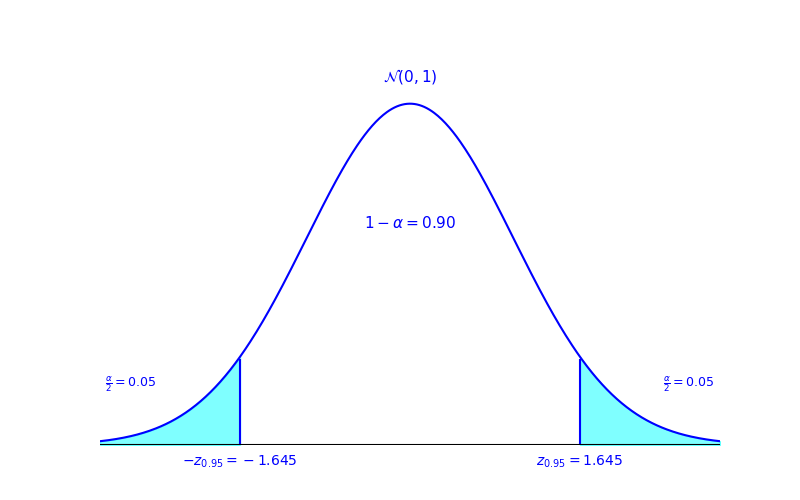
\includegraphics[width=\linewidth]{Tema 3/figures/Figure 3}
\end{minipage}
$\begin{array}{l}
    \overline{x}=20.02\\
1-\alpha=0.09\\
\alpha=0.1\\
\dfrac{\alpha}{2}=0.05\\
\left(20.2\mp 1.645 \dfrac{0.05}{\sqrt{5} }\right)=(20.02\mp 0.0367) = (19.9833, 20.0588)
\end{array}$

\subsection{Comentarios importantes}
\begin{tcolorbox}[colback=olive!5!white, colframe=olive!75!black, title=\textbf{Si $X$ no es Normal}]
\begin{itemize}[label=\textbullet]
    \item Hemos trabajado con la hipótesis de que $X$ es Normal para encontrar el estadístico pivotal $\dfrac{\overline{X}-\mu}{\sigma / \sqrt{n} }\sim \mathcal{N}(0,1)$.
    \item Si $X$ no es Normal, no podemos garantizar la confianza especificada.
    \item Sin embargo, si $n$ grande, tenemos por el Teorema Central del Límite \[
    \dfrac{\overline{X}-\mu}{\sigma / \sqrt{n} }\sim \mathcal{N}(0,1),\text{ aproximiadamente, }
    \] 
    entonces la confianza especificada no será exacta pero casi\dots
\end{itemize}
\end{tcolorbox}
\subsubsection{Factores que afectan a la precisión de la estimación}
\begin{tcolorbox}[colback=olive!5!white, colframe=olive!75!black, title=\textbf{El margen de error es $z_{1-\alpha /2}\dfrac{\sigma}{\sqrt{n} }$.}]
\begin{itemize}[label=\textbullet]
    \item $n\uparrow\longrightarrow \text{ precisión }\uparrow$
    \item $\sigma\uparrow\longrightarrow \text{ precisión }\downarrow$ 
    \item Confianza $\uparrow\longrightarrow $ precisión $\downarrow$
\end{itemize}
\end{tcolorbox}
\subsubsection{Determinación del tamaño muestral}
\begin{tcolorbox}[colback=blue!5!white, colframe=blue!75!black, title=\textbf{Contexto}]
Antes de extraer la muestra:
\begin{itemize}[label=\textbullet]
    \item Tenemos decidido el valor de $\sigma$.
    \item Tenemos decidido la confianza con la que trabajamos.
    \item Tenemos decidio el margen de error máximo $max$ que estamos dispuestos a comenter.
\end{itemize}
¿Qué tamaño de la muestra debemos escoger?
\end{tcolorbox}
Margen de error: $z_{1-\alpha /2}\dfrac{\sigma}{\sqrt{n} }\le max.\longrightarrow $ Despejamos $n$
\subsubsection{Otros modelos, estadísticos pivotales}
 \begin{tcolorbox}[colback=blue!5!white, colframe=blue!75!black, title=\textbf{$X\sim \mathcal{N}(\mu,\sigma^2)$, estimamos $\mu,\sigma$ desconocida}]
Estadístico pivotal: \[
T=\dfrac{\overline{X}-\mu}{S / \sqrt{n} }\sim t_{n-1}
\] 
\end{tcolorbox}

Debemos encontrar valores $a$ y $b$ tales que:

\begin{minipage}{0.45\textwidth}
    \includegraphics[width=\linewidth]{"Tema 3/figures/Figure 4"}
\end{minipage}$\begin{array}{l}
    P\left[ a\le \dfrac{\overline{X}-\mu}{S / \sqrt{n} }\le b \right] \\
    P\left[ -t_{n-1,1-\frac{\alpha}{2}}\le \dfrac{\overline{X}-\mu}{S / \sqrt{n} }\le t_{n-1,1-\frac{\alpha}{2} } \right] \\
    P\left[ X-t_{n-1,1-\frac{\alpha}{2} }\dfrac{S}{\sqrt{n} }\le \dfrac{\overline{X}-\mu}{S / \sqrt{n} }\le X+t_{n-1,1-\frac{\alpha}{2} }\dfrac{S}{\sqrt{n} } \right] =1-\alpha
\end{array}$

Obteniendo como I.C aleatorio a nivel $100(1-\alpha)\%$ \[
X-t_{n-1,1-\frac{\alpha}{2} }\dfrac{S}{\sqrt{n} }
\] 
\begin{tcolorbox}[colback=blue!5!white, colframe=blue!75!black, title=\textbf{$X\sim \mathcal{N}(\mu,\sigma^2)$, estimamos $\sigma^2$}]
Estadístico pivotal: \[
\dfrac{(n-1)S_n^2}{\sigma^2}\sim \chi_{n-1}^2
\] 
\end{tcolorbox}
I.C para $\sigma^2$ al nivel de confianza $(1-\alpha)100\%$ \[
T=\dfrac{(n-1)s^2}{\sigma^2}\leadsto \chi_{n-1}^2
\] 
Debemos encontrar valores $a$ y $b$ tales que: $P\left[ a\le \dfrac{(n-1)s^2}{\sigma^2}\le b \right]=1-\alpha $

\begin{minipage}{0.45\textwidth}
    \includegraphics[width=\linewidth]{"Tema 3/figures/Figure 5"}
\end{minipage}
$\begin{array}{l}
    P\left[ -\chi_{n-1,\frac{1-\alpha}{2} }^2\le \dfrac{(n-1)s^2}{\sigma^2}\le \chi_{n-1,1-\frac{\alpha}{2} }^2 \right] =1-\alpha\\
    P\left[ -\dfrac{1}{\chi_{n-1,1-\frac{\alpha}{2}}} \le  \dfrac{\sigma^2}{(n-1)s^2}\le \dfrac{1}{\chi_{n-1,1-\frac{\alpha}{2} }^2} \right] =1-\alpha\\
    P\left[ -\dfrac{(n-1)s^2}{\chi_{n-1,1-\frac{\alpha}{2} }^2}\le \sigma^2\le \dfrac{(n-1)s^2}{\chi_{n-1,1-\frac{\alpha}{2} }^2} \right] =1-\alpha
\end{array}$


\newpage

\section{Análisis de componentes principales}
\subsection{Introducción}
\begin{enumerate}[label=\arabic*)]
	\item Objetivo
\end{enumerate}
Simplificar la representación de datos multidimensionales al transformarlos en un nuevo conjunto de variables llamadas \lb{componentes principales}.
\begin{itemize}
	\item \lb{Reducción de dimensionalidad:} a veces dispondremos de muchas variables y simplemente se querrá disminuir el número de variables perdiendo la menor información posible (\lb{compresión de datos}).
	\begin{itemize}
		\item Útil en aplicaciones de almacenamiento y transmisión de información.
	\end{itemize}
	\item \lb{Visualización de datos:} al proyectar los datos en un espacio de menor dimensión, es más fácil representar gráficamente la estructura subyacente de los datos, lo que puede ayudar a identificar patrones, agrupaciones o relaciones (\lb{extracción de características}).
	\item \lb{Eliminación de multicolinealidad:} en análisis de regresión y otros contextos, la multicolinealidad (alta correlación entre variables independientes) puede ser problemática.
	\begin{itemize}
		\item En estos casos puede ayudar a reducir la multicolinealidad el \lb{transformar las variables originales} en un conjunto de variables no correlacionadas (las \lb{componentes principales}).
	\end{itemize}
\end{itemize}
\begin{itemize}[label=\color{red}\textbullet, leftmargin=*]
	\item \color{lightblue}Planteamiento desde el punto de vista teórico
\end{itemize}
La idea es \lb{resumir la información} de un \vea (v.a.) $k$-dimensional $\mathbf{X}=(X_1,\dots,X_k)'$ (recordemos que $A'$ denota la traspuesta de $A$, es decir, $\mathbf{X}$ es un vector columna) en unas \lb{pocas variables} que proporcionen la información más relevante.

Se puede dar una aproximación geométrica mediante el concepto de \lb{elipsoide de concentración}.
\begin{itemize}[label=\color{red}\textbullet, leftmargin=*]
	\item \color{lightblue}Definición
\end{itemize}
Si $\mathbf{X}$ es un vector aleatorio de dimensión $k$, media $\mu$ y su matriz de covarianzas $V=(\sigma_{i,j})$ definida positiva, se define el \lb{elipsoide de concentración} de $\mathbf{X}$ como \[ E_k=\{\mathbf{x}\in\R^k:(\mathbf{x}-\mu)'V^{-1}(\mathbf{x}-\mu)\le k+2\}. \]
En la definición del elipsoide interviene la \lb{distancia de Mahalanobis basada en la matriz $V$} entre $\mathbf{x}$ y la media $\mu$ dada por \[ d_V(\mathbf{x},\mu)=\sqrt{(\mathbf{x}-\mu)'V^{-1}(\mathbf{x}-\mu)}. \]
Esta distancia al cuadrado se puede calcular en \code{R} con \code{mahalanobis(x, mu, V)}.

Además, si $X$ es \lb{normal}, el elipsoide se puede definir a partir de las \lb{curvas de nivel de la función de densidad} ($f(x)=cte$.) ya que \[ f(x)=\dfrac{1}{\sqrt{|V|(2\pi)^k}}\exp\left(-\dfrac{1}{2}(\mathbf{x}-\mu)'V^{-1}(\mathbf{x}-\mu)\right). \]
Una parte de los individuos (puntos estarán dentro de este elipsoide).

Si queremos \lb{distinguirlos con una única variable}, parece claro que lo mejor sería proyectarlos sobre el eje mayor del elipsoide.

Por ejemplo, para una \lb{normal bivariante} \[ \mathcal{N}_2\left(\mu=\binom{0}{0},V=\begin{pmatrix}
	1 & \tfrac{1}{2}\\
	\tfrac{1}{2} & 1
\end{pmatrix}\right) \] se tiene que \[ (x_1,x_2)\begin{pmatrix}
1 & \tfrac{1}{2}\\
\tfrac{1}{2} & 1
\end{pmatrix}^{-1}\binom{x_1}{x_2}=\dfrac{4}{3}x_1^2-\dfrac{4}{3}x_1x_2+\dfrac{4}{3}x_2^2 \] por lo que el \lb{elipsoide de concentración} sería \[ \dfrac{4}{3}x_1^2-\dfrac{4}{3}x_1x_2+\dfrac{4}{3}x_2^2\le4 \]

\begin{itemize}
	\item \lb{Elipsoide de concentración} para la normal bivariante con medias 0, varianzas 1 y correlación $\dfrac{1}{2}:$
	
	\begin{lstlisting}
hc <- function(x1, x2) (4/3)*x1^ 2- (4/3)*x1*x2 + (4/3)*x2^ 2
x1 <- seq(-3, 3, length =1000)
x2 <- seq(-3, 3, length =1000)
z <- outer(x1, x2, hc)
contour(x1, x2, z, levels = 4)
title(main = "level = 4")
	\end{lstlisting}
	\begin{center}
		\includegraphics[width=0.5\linewidth]{"Temas/Imágenes/Tema 4/screenshot001"}
	\end{center}
	\item \lb{Elipsoides obtenidos con otros niveles} (circunferencias de Mahalanobis):
	\begin{lstlisting}
hc <- function(x1, x2) (4/3)*x1^ 2- (4/3)*x1*x2 + (4/3)*x2^ 2
x1 <- seq(-3, 3, length =1000)
x2 <- seq(-3, 3, length =1000)
z <- outer(x1, x2, hc)
contour(x1, x2, z, levels = c(1:6))
title(main = "level = 1, ..., 6")
	\end{lstlisting}
	\begin{center}
		\includegraphics[width=0.5\linewidth]{"Temas/Imágenes/Tema 4/screenshot002"}
	\end{center}
\end{itemize}

\begin{minipage}{0.45\textwidth}
	Si queremos \lb{reducir las dos variables a solo una}, la mejor proyección, es decir la que mejor separa los puntos (\lb{varianza máxima}), es la proporcionada por el \lb{eje principal del elipsoide} (o curvas de nivel de la normal).
	
	En este ejemplo viene dado por la recta: \[ x_2=x_1. \]
\end{minipage}\qquad\begin{minipage}{0.5\textwidth}
\begin{lstlisting}
hc <- function(x1, x2) (4/3)*x1^ 2- (4/3)*x1*x2 + (4/3)*x2^ 2
x1 <- seq(-3, 3, length =1000)
x2 <- seq(-3, 3, length =1000)
z <- outer(x1, x2, hc)
contour(x1, x2, z, levels = c(1:6))
abline(a = 0, b = 1, col = "red", lty = 2)
abline(a = 0, b = -1, col = "blue", lty = 2)
title(main = "level = 1, ..., 6")
\end{lstlisting}
\end{minipage}
\begin{flushright}
\includegraphics[width=0.5\linewidth]{"Temas/Imágenes/Tema 4/screenshot003"}
\end{flushright}
\begin{itemize}[label=\color{red}\textbullet, leftmargin=*]
	\item \color{lightblue}Objetivo
\end{itemize}
\lb{Transformar} un conjunto de $k$ variables interrelacionadas entre sí en un nuevo conjunto con un número menor de variables:
\begin{itemize}
	\item las \lb{componentes principales}
\end{itemize}
De manera que estas nuevas variables:
\begin{itemize}
	\item sean \lb{ortogonales entre sí}.
	\item capturen la \lb{mayor variabilidad} de las variables.
	\item \lb{expliquen la mayor parte de la variabilidad} de las variables originales.
\end{itemize}
\begin{itemize}[label=\color{red}\textbullet, leftmargin=*]
	\item \color{lightblue}Planteamiento teórico
\end{itemize}
Supongamos que $\mathbf{X}=(X_1,\dots,X_k)'$ es un \vea $k$-dimensional con vector de medias $\mu$ y matriz de covarianzas $V$ \lb{semidefinida positiva}.

Entonces la \lb{primera componente principal} será la \va unidimensional \[ Y_1=a_1X_1+\cdots+a_kX_k \] con $a_1^2+\cdots+a_k^2=1$ cuya \lb{varianza es máxima}.
\begin{itemize}
	\item Si no se normaliza la combinación lineal, la variable $Y_1$ puede tener varianza tan grande como queramos.
	\item Geométricamente, hacemos un cambio de variable (primer eje) para que la dispersión sea máxima y la normalización equivale a mantener la escala original (proyectar).
\end{itemize}
El problema puede expresarse de la forma siguiente: \[ \begin{rcases}
	\max&\var(a'\mathbf{X})\\
	\text{s.a.} & \mathbf{a'a}=1
\end{rcases} \] donde $\mathbf{a}=(a_1,\dots,a_k)'\in\R^k$.

Una vez calculada una primera componente principal $Y_1$, la \lb{segunda componente principal} $Y_2$ debe verificar $\cov(Y_1,Y_2)=0$ (no debe contener información ya incluida en $Y_1$) y debe tener la \lb{varianza máxima}, es decir, \[ \begin{rcases}
	\max & \var(\mathbf{a'X})\\
	\text{s.a.} & \mathbf{a'a}=1\\
	&\cov(Y_1,\mathbf{a'X})=0
\end{rcases} \]
Así, sucesivamente, por inducción, se definen las \lb{siguientes componentes principales} $(Y_j)$ como la (una) solución de 
\[ \begin{rcases}
	\max & \var(\mathbf{a'X})\\
	\text{s.a.} & \mathbf{a'a}=1\\
	&\cov(Y_1,\mathbf{a'X})=0,\quad i=1,\dots,j-1
\end{rcases} \]
\begin{itemize}[label=\color{lightblue}\textbullet]
	\item La solución general viene dada en el teorema siguiente que prueba la \lb{existencia de las (unas) componentes principales} y muestra \lb{cómo calcularlas}.
	\item Además, se demuestra que las componentes principales \lb{no son únicas} (puede haber más soluciones).
\end{itemize}
\begin{itemize}[label=\color{red}\textbullet, leftmargin=*]
	\item \color{lightblue}Teorema de existencia
\end{itemize}
Si $\mathbf{X}$ es un \vea $k$-dimensional con matriz de covarianzas $V$ \lb{definida positiva}, las (unas) \lb{componentes principales} se obtienen como \[ \mathbf{Y}=(Y_1,\dots,Y_k)'=T'\mathbf{X}=\begin{pmatrix}
	t_{1,1} & \cdots & t_{k,1} \\
	\cdots & \cdots & \cdots \\
	t_{1,k} & \cdots & t_{k,k}
\end{pmatrix}\begin{pmatrix}
X_1\\
\cdots\\
X_k
\end{pmatrix}, \] donde $T$ es una \lb{matriz ortogonal} $(T'T=TT'=I)$ tal que \[ T'VT=D=\mathrm{diag}(\lambda_1,\dots,\lambda_k) \]con $\lambda_1\ge\lambda_2\ge\cdots\ge\lambda_k>0$.
\begin{itemize}[label=\color{red}\textbullet, leftmargin=*]
	\item \color{lightblue}Demostración
\end{itemize}
Como $V$ es una matriz \lb{simétrica} y \lb{definida positiva}, existe una matriz $T=(t_{i,j})$ \lb{ortogonal} $(T'T=TT'=I)$ tal que \[ T'VT=D=\mathrm{diag}(\lambda_1,\dots,\lambda_k) \] con los valores propios verificando $\lambda_1\ge\lambda_2\ge\cdots\ge\lambda_k>0$.

De esta forma, si \[ \mathbf{Y}=(Y_1,\dots,Y_k)'=T'\mathbf{X}=\begin{pmatrix}
	t_{1,1} & \cdots & t_{k,1} \\
	\cdots & \cdots & \cdots \\
	t_{1,k} & \cdots & t_{k,k}
\end{pmatrix}\begin{pmatrix}
	X_1\\
	\cdots\\
	X_k
\end{pmatrix} \] entonces $Y_1,\dots,Y_k$ verifican que \[ \cov(\mathbf{Y})=\cov(T'\mathbf{X})=E[T'(\mathbf{X-\mu})(\mathbf{X}-\mu)'T]=T'VT=D, \]lo que indica que $\cov(Y_i,Y_j)=0$ para $i\neq j$ y $\var(Y_j)=\lambda_j$.

Para comprobar que $Y_1$ es una primera componente principal, supongamos que $\mathbf{a'X}$ es una combinación lineal con $\mathbf{a'a}=1$.

Las columnas de la matriz $T$ corresponden a los vectores propios $\mathbf{t}_i$ asociados a los autovalores $\lambda_i,T=(\mathbf{t}_1|\cdots|\mathbf{t}_k)$, y como los vectores propios son una base, existirán $c_1,\dots,c_k$ números reales tales que \[ \mathbf{a}=c_1\mathbf{t}_1+\cdots+c_k\mathbf{t}_k=\sum_{i=1}^{k}c_i\mathbf{t}_i. \]
Con lo que 
\begin{align*}
	\var(\mathbf{a'X})&=E[\mathbf{a'(X-\mu)(X-\mu)'a}]=\mathbf{a}'\cov(\mathbf{X})\mathbf{a}=\mathbf{a'}V\mathbf{a}\\
	&=\left(\sum_{i=1}^{k}c_i\mathbf{t}_i'\right)V\left(\sum_{i=1}^{k}c_i\mathbf{t}_i\right)=\left(\sum_{i=1}^{k}c_i\mathbf{t}_i'\right)\left(\sum_{j=1}^{k}c_jV\mathbf{t}_j\right)\\
	&=\left(\sum_{i=1}^{k}c_i\mathbf{t}_i'\right)\left(\sum_{j=1}^{k}c_j\lambda_j\mathbf{t}_j\right)=\sum_{i,j}c_ic_j\lambda_j\mathbf{t}_i'\mathbf{t}_j=\sum_{i=1}^{k}c_i^2\lambda_i
\end{align*}
Y, como \[ \mathbf{a'a}=\left(\sum_{i=1}^{k}c_i\mathbf{t}_i'\right)\left(\sum_{j=1}^{k}c_j\mathbf{t}_j\right)=\sum_{i,j}c_ic_j\mathbf{t}_i'\mathbf{t}_j=\sum_{i=1}^{k}c_i^2=\mathbf{c'c}=1, \] con $\mathbf{c}=(c_1,\dots,c_k)'$, la varianza será máxima si $x_1^2=1,c_2=0,\dots,c_k=0$ ya que \[ \var(\pm\mathbf{t}_1'\mathbf{X})=\lambda_1=\mathbf{c'c}\lambda_1=\sum_{i=1}^{k}c_i^2\lambda_1\ge\sum_{i=1}^{k}c_i^2\lambda_i=\var(\mathbf{a'X}), \]para todo $\mathbf{a}$ tal que $\mathbf{a'a}=1$, es decir, $Y_1=\pm \mathbf{t}_1'\mathbf{X}$ es una primera componente principal (puede haber otras soluciones si $\lambda_1=\lambda_2$).

Por inducción, supongamos que $Y_1=\mathbf{t}_1'\mathbf{X},\dots,Y_{j-1}\mathbf{X}$ son las primeras ($j-1$) componentes principales.

Y veamos que $Y_j=\mathbf{t}_j'\mathbf{X}$ es la (una) solución de \[ \begin{rcases}
	\max & \var(\mathbf{a'X})\\
	\text{s.a.} & \mathbf{a'a}=1\\
	&\cov(Y_1,\mathbf{a'X})=0,\quad i=1,\dots,j-1
\end{rcases} \]
Como se debe verificar \begin{align*}
	\cov(\mathbf{a'X},Y_i) & = \cov(\mathbf{a'X},\mathbf{t}_i'\mathbf{X})=E[\mathbf{a'(X-\mu)(X-\mu)'t}_i]=\mathbf{a}'\cov(\mathbf{X})\mathbf{t}_i\\
	&=\mathbf{a'}V\mathbf{t}_i=\mathbf{a'\lambda}_i\mathbf{t}_i=\lambda_i\mathbf{a't}_i=\lambda_i\left(\sum_sc_s\mathbf{t}_s'\right)\mathbf{t}_i=\lambda_ic_i=0
\end{align*} para $i=1,\dots,j-1,\:\lambda_i>0$, se tiene $c_1=\cdots=c_{j-1}=0$.

Entonces, la varianza será máxima si $c_j=1$ y $c_i=0$ para $i>j$, ya que \[ \var(\pm\mathbf{t}_j'\mathbf{X})=\lambda_j=\mathbf{c'c}\lambda_j=\sum_{i=j}^{k}c_i^2\lambda_j\ge\sum_{i=j}^{k}c_i^2\lambda_i=\var(\mathbf{a'X}), \] para todo $\mathbf{a}$ tal que $\mathbf{a'a}=1$ y $\cov(\mathbf{a'X}, Y_i)=0,\:i=1,\dots,j-1$, es decir, $Y_j=\pm\mathbf{t}_j'\mathbf{X}$ es una componente principal $j$-ésima (no necesariamente la única).

\begin{itemize}[label=\color{red}\textbullet, leftmargin=*]
	\item \color{lightblue}Corolario
\end{itemize}
Si $\lambda_1>\lambda_2>\cdots>\lambda_k$, entonces las componentes principales son únicas salvo digno.
\begin{itemize}[label=\color{red}\textbullet, leftmargin=*]
	\item \color{lightblue}Observación
\end{itemize}
Nótese que la componente principal $j$-ésima se obtiene multiplicando la fila $j$-ésima de $T'$ (la columna $j$-ésima de $T$) por $\mathbf{X}$, es decir, \[ Y_j=\mathbf{t}_j'\mathbf{X} \]donde $\mathbf{t}_j'=(t_{1,j},\dots,t_{k,j})$ es un vector propio unitario correspondiente al $j$-ésimo valor propio (vectores columna de $T$).

Además, $\var(Y_j)=\lambda_j$, y \[ \mathrm{traza}(V)=\sum_{j=1}^{k}\sigma_{j,j}=\sum_{j=1}^{k}\var(X_j)=\sum_{j=1}^{k}\var(Y_j)=\sum_{j=1}^{k}\lambda_j \](las matrices semejantes tienen las trazas iguales), es decir, la \lb{variabilidad} (información) de las variables originales es igual a la suma de las variabilidades de las componentes principales.

La \lb{cantidad de información} (\%) contenida en cada componente será \[ I_j=100\dfrac{\lambda_j}{\displaystyle\sum_{i=1}^{k}\lambda_i}\%. \]
Por esto, la \lb{traza} se usar como una medida unidimensional de la dispersión de una variable $k$-dimensional.

La otra medida es el \lb{determinante} de $V$ para el que también se verifica: \[ |V|=\lambda_1\cdots\lambda_k=|\cov(\mathbf{Y})| \]
\begin{itemize}[label=\color{red}\textbullet, leftmargin=*]
	\item \color{lightblue}Observación
\end{itemize}
Otros autores llaman componentes principales a \[ \mathbf{Y}=T'(\mathbf{X-\mu}) \] con lo que, además, se consigue que sean centradas ($E[Y_j]=0$),
\begin{itemize}
	\item \lb{compronentes principales centradas}
\end{itemize}
También se pueden definir las \lb{componentes principales estandarizadas} \[ Z_j=\mathbf{t}_j'(\mathbf{X-\mu})\lambda_j^{-\frac{1}{2}} \] $(\mathbf{Z}=D^{-\frac{1}{2}}T'(\mathbf{X-\mu}))$ que además de ser centradas tendrán varianza 1.

Cuando hay \lb{valores propios iguales a cero} ($V$ es \lb{semidefinida positiva}) no suelen considerarse sus correspondientes componentes principales (degeneradas) y se puede conservar toda la información en las componentes principales de valores propios distintos de cero.

En este caso hay \lb{variables} que pueden obtenerse como \lb{combinación lineal de las restantes} (aunque no siempre pueden eliminarse del análisis).

Geométricamente, las \lb{componentes principales} se corresponden con los \lb{ejes principales del elipsoide de concentración}.

Como $\mathbf{Y}=T'\mathbf{X}$, podemos interpretar las componentes en función de los pesos que tengan en ellas las variables originales.

Si ponemos $\mathbf{X}$ en función de $\mathbf{Y}$ como $\mathbf{X}=T\mathbf{Y}$, entonces las variables originales se pueden interpretar en función de las componentes principales e incluso, podemos representar aproximadamente, las variables originales usando las dos (tres) primeras componentes.
\begin{itemize}[label=\color{red}\textbullet, leftmargin=*]
	\item \color{lightblue}Caso de normalidad
\end{itemize}
Si la población $\mathbf{X}$ es \lb{normal}, entonces las \lb{componentes principales} son \lb{normales} e \lb{independientes entre sí}, ya que en estas poblaciones equivalen los conceptos de independencia e incorrelación (independencia lineal) y $\mathbf{Z}$ será una normal estándar multivariante ($\mathcal{N}_k(0,I)$).
\begin{itemize}[label=\color{red}\textbullet, leftmargin=*]
	\item \color{lightblue}Proposición
\end{itemize}
Si $\mathbf{Y}$ son las \lb{componentes principales} obtenidas a partir de $\mathbf{X}$, entonces $\mathbf{X}$ es \lb{normal multivariante} si, y sólo si $Y_1,\dots,Y_k$ son \lb{independientes} y \lb{normales univariantes} para todo $j=1,\dots,k$.
\begin{itemize}[label=\color{red}\textbullet, leftmargin=*]
	\item \color{lightblue}Demostración.
\end{itemize}
La demostración es inmediata.

Esta propiedad puede ser utilizada para estudiar la normalidad multivariante a partir de un test de normalidad univariante sobre las componentes principales.

Incluso si la normal multivariante no es de rango completo ($V$ no es definida positiva), puede utilizarse con con las $m$ primeras componentes con valores propios distintos de cero (las otras serán degeneradas) coincidiendo $m$ con el rango de $V$.

\Ej

Para el \vea normal de media $\mu=(0,0)$ y matriz de covarianzas $V=\begin{pmatrix}
	1 & \tfrac{1}{2}\\
	\tfrac{1}{2} & 1
\end{pmatrix}$

\hspace{1cm}

\begin{lstlisting}
library("mvtnorm")
f <- function(x1, x2) dmvnorm(data.frame(x1, x2), mu, V)
V <- matrix(c(1, 1/2,
1/2, 1), nrow = 2, ncol = 2, byrow = TRUE)
mu <- c(0, 0)
x1 <- seq(-3, 3, length = 50)
x2 <- seq(-3, 3, length = 50)
z <- outer(x1, x2, f)
persp(x1, x2, z, xlab = 'x1', ylab = 'x2', zlab = 'f(x1, x2)', col = 'orange', main = "Función de densidad")
\end{lstlisting}
\begin{center}
	\includegraphics[width=0.6\linewidth]{"Temas/Imágenes/Tema 4/screenshot004"}
\end{center}

\pagebreak

\begin{lstlisting}
#Se fija la semilla para la generación aleatoria
set.seed(123)
d <- rmvnorm(50, mu, V)
plot(d, xlab = "X1", ylab = "X2", pch = 20, xlim = c(-3, 3), ylim = c(-3, 3), main = "Elipsoide de concentración")
hc <- function(x1, x2) (4/3)*x1^ 2 - (4/3)*x1*x2 + (4/3)*x2^ 2
x1 <- seq(-3, 3, length = 1000)
x2 <- seq(-3, 3, length = 1000)
z <- outer(x1, x2, hc)
contour(x1, x2, z, levels = 4, add = T, col = 'red')
\end{lstlisting}
\begin{center}
	\includegraphics[width=0.6\linewidth]{"Temas/Imágenes/Tema 4/screenshot005"}
\end{center}
Sus componentes principales se calcularán diagonalizando $V$ mediante \[ \left|V-\lambda I\right|=\begin{vmatrix}
	1-\lambda & 0.5\\
	0.5 & 1-\lambda
\end{vmatrix}=1-2\lambda+\lambda^2-\dfrac{1}{4}=0 \] que tiene soluciones \[ \lambda=\dfrac{2\pm\sqrt{4-4(1-\frac{1}{4})}}{2}=1\pm0.5, \]$\lambda_1=1.5$ y $\lambda_2=0.5$.

Y la \lb{primera componente} se obtendrá resolviendo $V\mathbf{v}=\lambda\mathbf{v}$ \[ \begin{pmatrix}
	1 & 0.5\\
	0.5 & 1
\end{pmatrix}\begin{pmatrix}
x_1\\
x_2
\end{pmatrix}=1.5\begin{pmatrix}
x_1\\
x_2
\end{pmatrix}\xRightarrow{\qquad}\begin{pmatrix}
-0.5x_1+0.5x_2\\
0.5x_1-0.5x_2
\end{pmatrix}=\begin{pmatrix}
0\\
0
\end{pmatrix} \]lo que da $x_1=x_2$, es decir, sus vectores propios son de la forma $\mathbf{v}=\alpha(1,1)'$.

Como usamos vectores normalizados (de norma 1), una primera componente valdrá \[ Y_1=\left(\dfrac{1}{\sqrt{2}},\dfrac{1}{\sqrt{2}}\right)\dbinom{X_1}{X_2}=\dfrac{X_1+X_2}{\sqrt{2}} \]y su varianza es $\lambda_1=1.5$.

Análogamente, la segunda valdrá $Y_2=\dfrac{X_1-X_2}{\sqrt{2}}$ (ya que tiene que ser perpendicular a la primera) y tendrá varianza $\lambda_2=0.5$.

Es decir, tenemos \[ \begin{array}{l}
	Y_1=\dfrac{X_1+X_2}{\sqrt{2}}\\
	Y_2=\dfrac{X_1-X_2}{\sqrt{2}}\\
\end{array} \]por lo que \[ \mathbf{Y}=T'\mathbf{X}=\begin{pmatrix}
\frac{1}{\sqrt{2}} & \frac{1}{\sqrt{2}}\\
\frac{1}{\sqrt{2}} & -\frac{1}{\sqrt{2}}\\
\end{pmatrix}\begin{pmatrix}
X_1\\
X_2
\end{pmatrix}. \]
\lb{Varianza total explicada} por cada componente:
\begin{itemize}
	\item La primera componente explicará un 75\% de la varianza total: \[ I_1=100\dfrac{\lambda_1}{\lambda_1+\lambda_2}\%=75\%. \]
	\item La segunda un 25\% de la varianza total: \[ I_2=100\dfrac{\lambda_2}{\lambda_1+\lambda_2}\%=25\%. \]
\end{itemize}
Como las varianzas iniciales son iguales, ambas tienen igual peso en las componentes con distinto signo en el caso de la segunda de ellas.

Aunque las varianzas iniciales sean todas iguales (1) las componentes principales tienen varianzas (en general) distintas.

Si $X_1$ fuese el peso de una persona y $X_2$ su altura (estandarizadas).
\begin{itemize}
	\item La primera componente se podría interpretar como lo \lb{grande} que es dicha persona.
	\item Mientras que la segunda estará relacionada con su \lb{constitución} ($Y_2$ grande significaría mucho peso y poca altura, es decir, complexión fuerte).
\end{itemize}
Despejando, se tiene \[ \begin{array}{l}
	X_1=\dfrac{Y_1+Y_2}{\sqrt{2}}\\
	X_2=\dfrac{Y_1-Y_2}{\sqrt{2}}\\
\end{array} \] lo que nos permite representar las variables $X_1,\:X_2$ en función de las componentes $Y_1,\:Y_2$.
\begin{itemize}
	\item $Y_1$ aumenta si lo hacen $X_1$ y $X_2$.
	\item $Y_2$ aumenta si aumenta $X_1$ y disminuye $X_2$.
	\item Estas relaciones servirán para interpretar (dar significado) a las componentes principales.
\end{itemize}
\subsection{¿Cómo realizamos estos cálculo en \textbf{\texttt{R}}?}
En primer lugar definimos e introducimos $V$
\begin{lstlisting}
V <- matrix(c(1, 1/2, 1/2, 1), nrow = 2, ncol = 2, byrow = TRUE)
V
\end{lstlisting}
\begin{verbatim}
##      [,1] [,2]
## [1,]  1.0  0.5
## [2,]  0.5  1.0
\end{verbatim}
Calculamos los valores y vectores propios:
\begin{lstlisting}
eigen(V)$values; eigen(V)$vectors
\end{lstlisting}
\begin{verbatim}
## [1] 1.5 0.5
##           [,1]       [,2]
## [1,] 0.7071068 -0.7071068
## [2,] 0.7071068  0.7071068
\end{verbatim}
Podemos guardar la matriz $T$ de vectores propios:
\begin{lstlisting}[mathescape=false]
T <- eigen(V)$vectors
\end{lstlisting}
Los vectores normalizados aparecen en las columnas de $T$. Podemos comprobar que $T$ es una matriz ortogonal:
\begin{lstlisting}
t(T) %*% T
\end{lstlisting}
\begin{verbatim}
##      [,1] [,2]
## [1,]    1    0
## [2,]    0    1
\end{verbatim}
donde \code{t(A)} es la traspuesta de \code{A} y \code{A \%*\% B} es el producto de las matrices \code{A} y \code{B} en \code{R}.

Podemos comprobar que $T$ diagonaliza a $V$:
\begin{lstlisting}
t(T) %*% V %*% T
\end{lstlisting}
\begin{verbatim}
##      [,1] [,2]
## [1,]  1.5  0.0
## [2,]  0.0  0.5
\end{verbatim}
lo que nos dará la matriz diagonal con los valores 1.5 y 0.5 en la diagonal.

Como $\mathbf{Y}=T'\mathbf{X}$, las componentes principales serán \[ \begin{array}{l}
	Y_1=0.7071068X_1+0.7071068X_2=\dfrac{X_1+X_2}{\sqrt{2}}\\
	Y_2=-0.7071068X_1+0.7071068X_2=-\dfrac{X_1+X_2}{\sqrt{2}}\\
\end{array} \]
Para calcular las informaciones contenidas en cada una (en tanto por 100) haremos:
\begin{lstlisting}
100*eigen(V)$values/sum(eigen(V)$values)
\end{lstlisting}
\begin{verbatim}
## [1] 75 25
\end{verbatim}
obteniendo el 75\% y el 25\%
\subsection{Desigualdades}
Si $Z$ es una variable aleatoria no negativa con media finita $E[Z]$ y $\epsilon>0$, entonces \[ \epsilon Pr[Z\ge\epsilon]=\epsilon\int_{[\epsilon,\infty)}\mathrm{d}F_Z(x)\le\int_{[\epsilon,\infty)}x\mathrm{d}F_Z(x)\le\int_{[0,\infty)}x\mathrm{d}F_Z(x)=E(Z) \] (donde $F_Z(x)=Pr[Z\le x]$ es su función de distribución), es decir \[ Pr[Z\ge \epsilon]\le\dfrac{E[Z]}{\epsilon}. \]

$\bboxed{E\left[\dfrac{(X-\mu)^2}{\sigma^2}\right]=\dfrac{1}{\sigma^2}E[(X-\mu)^2]=\dfrac{\sigma^2}{\sigma^2}=1}$

Si $X$ es una variable aleatoria con media finita $\mu=E[X]$ y varianza $\sigma^2=\var(X)>0$, entonces tomando $Z=\dfrac{(X-\mu)^2}{\sigma^2}\ge0$ y aplicando la desigualdad de Markov, tenemos \[ Pr\left[\dfrac{(X-\mu)^2}{\sigma^2}\ge\epsilon\right]\le\dfrac{1}{\epsilon} \]para todo $\epsilon>0$.
\subsubsection{Desigualdad de Chebyshev}
También se puede escribir como \[ Pr[(X-\mu)^2<\epsilon\sigma^2]\ge1-\dfrac{1}{\epsilon}, \] o como \[ Pr[|X-\mu|<r]\ge1-\dfrac{\sigma^2}{r^2}, \] para todo $r>0$.
\subsubsection{Desigualdad de Chebyshev multivariante}
Sea $\mathbf{X}=(X_1,\dots,X_k)'$ un \vea con vector de medias finito $\mu=E(\mathbf{X})$ y matriz de covarianzas definida positiva $V$, entonces \[ Pr[(\mathbf{X}-\mu)'V^{-1}(\mathbf{X}-\mu)\ge\epsilon]\le\dfrac{k}{\epsilon} \]para todo $\epsilon>0$.
\begin{itemize}[label=\color{red}\textbullet, leftmargin=*]
	\item \color{lightblue}Consecuencias
\end{itemize}
La desigualdad también se puede escribir como \[ Pr[(\mathbf{X}-\mu)'V^{-1}(\mathbf{X}-\mu)<\epsilon]\ge1-\dfrac{k}{\epsilon}, \] para todo $\epsilon>0$.

En particular, para el elipsoide de concentración \[ E_k=\{x\in\R^k:(\mathbf{X}-\mu)V^{-1}(\mathbf{X}-\mu)\le k+2\}, \] obtenemos \[ Pr[\mathbf{X}\in E_k]\ge1-\dfrac{k}{k+2}=\dfrac{2}{k+2}. \]
Para obtener regiones con más datos podemos tomar $\epsilon=ck$, resultando \[ Pr[(\mathbf{X}-\mu)'V^{-1}(\mathbf{X}-\mu)<ck]\ge1-\dfrac{k}{\epsilon}=1-\dfrac{1}{c}=\dfrac{c-1}{c}. \]
La \va no negativa $Z=(\mathbf{X}-\mu)'V^{-1}(\mathbf{X}-\mu)$ se puede escribir como \[ (\mathbf{X}-\mu)'TD^{-1}T'(\mathbf{X}-\mu)=\left[D^{-\frac{1}{2}}T'(\mathbf{X}-\mu)\right]'[D^{-\frac{1}{2}}T'(\mathbf{X}-\mu)]=\mathbf{Z'Z}, \] donde $\mathbf{Z}=D^{-\frac{1}{2}}T'(\mathbf{X}-\mu)\:(\mathbf{Z}=(Z_1,\dots,Z_k)')$.

Si $X$ es \lb{normal}, entonces $Z_1,\dots,Z_k$ son normales estándar independientes y \[ Z=\sum_{i=1}^{k}Z_i^2 \]sigue una \lb{distribución chi-cuadrado} con $k$ grados de libertad (ya que es la suma de $k$ normales $\mathcal{N}(0,1)$ independientes).
\subsection{Propiedades}
\begin{itemize}[label=\color{red}\textbullet, leftmargin=*]
	\item \color{lightblue}Proposición
\end{itemize}
Si $\mathbf{Y}$ son las componentes principales obtenidas a partir de $\mathbf{X}$, entonces \[ \begin{array}{l}
	\cov(\mathbf{X,Y})=TD\\
	\corr(\mathbf{X,Y})=\mathrm{diag}(V)^{-\frac{1}{2}}TD^{\frac{1}{2}}
\end{array} \] donde $\mathrm{diag}(V)=\mathrm{diag}(\sigma_1^2,\dots,\sigma_k^2)$.
\begin{itemize}[label=\color{red}\textbullet, leftmargin=*]
	\item \color{lightblue}Demostración
\end{itemize}
En primer lugar señalaremos que \[ \cov(\mathbf{X,Y})=\cov(\mathbf{X},T'\mathbf{X})=VT \] y, como $T'VT=D$ y $T$ es ortogonal, entonces $VT=TD$ y $\cov(\mathbf{X,Y})=TD$.

Por otro lado se tiene que como \[ \corr(X_i,Y_j)=\dfrac{\cov(X_i,Y_j)}{\sigma_i\lambda_j^{\frac{1}{2}}}, \]entonces \[ \corr(\mathbf{X,Y})=\mathrm{diag}(V)^{-\frac{1}{2}}\cov(\mathbf{X,Y})D^{-\frac{1}{2}} \]y\[ \corr(\mathbf{X,Y})=\mathrm{diag}(V)^{-\frac{1}{2}}TDD^{-\frac{1}{2}}=\mathrm{diag}(V)^{-\frac{1}{2}}TD^{\frac{1}{2}} \]
\begin{itemize}[label=\color{red}\textbullet, leftmargin=*]
	\item \color{lightblue}Corolario
\end{itemize}
En las condiciones de la proposición anterior se tiene: \[ \begin{array}{l}
	\cov(X_i,Y_j)=t_{i,j}\lambda_j\\
	\corr(X_i,Y_j)=\dfrac{t_{i,j}}{\sigma_i}\lambda_j^{\frac{1}{2}}
\end{array} \] para todo $i,j$.
\begin{itemize}[label=\color{red}\textbullet, leftmargin=*]
	\item \color{lightblue}Definición
\end{itemize}
Se denomina \lb{matriz de saturaciones} a \[ A=\corr(\mathbf{X,Y}). \]
\Ej

Para el \vea normal de media $\mu=(0,0)$ y matriz de covarianzas $V=\begin{pmatrix}
	1 & \tfrac{1}{2}\\
	\tfrac{1}{2} & 1
\end{pmatrix}$, se obtiene \[ T=(\mathbf{t}_1|\mathbf{t}_2)=\begin{pmatrix}
\frac{1}{\sqrt{2}} & \frac{1}{\sqrt{2}}\\
\frac{1}{\sqrt{2}} & -\frac{1}{\sqrt{2}}\\
\end{pmatrix},\quad D=\begin{pmatrix}
\lambda_1 & 0\\
0 & \lambda_2
\end{pmatrix}=\begin{pmatrix}
1.5 & 0\\
0 & 0.5
\end{pmatrix} \]por lo que la matriz de saturaciones valdrá: \[ A=\mathrm{diag}(V)^{-\frac{1}{2}}TD^{\frac{1}{2}}=\dfrac{1}{2}\begin{pmatrix}
\sqrt{3} & 1\\
\sqrt{3} & -1\\
\end{pmatrix}=\begin{pmatrix}
0.86603 & 0.5\\
0.86603 & -0.5\\
\end{pmatrix} \]

Nótese que:
\begin{itemize}
	\item La primera componente explica un 75\% (0.866\$\^\,2 \$ 100) de las variables $X_1$ y $X_2$.
	\item Mientras que la segunda solo un 25\%.
\end{itemize}
Las saturaciones y sus caudrados suelen representarse en tablas de la forma siguiente:
\[ \begin{array}{c|c|c}
	a_{i,j}=\corr(X_i,Y_j) & Y_1 & Y_2\\ \hline
	X_1 & 0.866 & 0.5\\ \hline
	X_2 & 0.866 & -0.5\\ \hline
\end{array}\qquad\begin{array}{c|c|c|c}
a_{i,j} & Y_1 & Y_2 & \text{Total}\\ \hline
X_1 & 0.75 & 0.25 & 1\\ \hline
X_2 & 0.75 & 0.25 & 1\\ \hline
\end{array} \] lo que nos puede ayudar a \lb{interceptar} las componentes principales.

Las saturaciones también se pueden representar gráficamente.

Aunque en este ejemplo, las saturaciones con las distintas variables coincidan, esto no siempre es así, y tendremos variables mejor explicadas por las componentes elegidas que otras.
\begin{itemize}[label=\color{red}\textbullet, leftmargin=*]
	\item \color{lightblue}Proposición
\end{itemize}
Si $A$ es la matriz de saturaciones, entonces \[ AA'=\corr(\mathbf{X}). \]
También es interesante calcular las correlaciones múltiples entre cada variable original con el grupo de las $p$ primeras componentes principales elegidas $(p\le k)$.
\begin{itemize}
	\item Para medir el máximo que podemos explicar de cada variable original a partir de combinaciones lineales de esas componentes principales.
\end{itemize}
\begin{itemize}[label=\color{red}\textbullet, leftmargin=*]
	\item \color{lightblue}Proposición
\end{itemize}
Si $\mathbf{Y}$ son las componentes principales obtenidas a partir de $\mathbf{X}$, entonces \[ \corr^2(X_i,(Y_1,\dots,Y_p))=\sum_{j=1}^{p}\corr^2(X_i,Y_j)=\dfrac{1}{\sigma_{i,i}}\sum_{j=1}^{p}t_{i,j}^2\lambda_j=\sum_{j=1}^{p}a_{i,j}^2. \]
La demostración es inmediata ya que las componentes son incorreladas entre sí.
\begin{itemize}[label=\color{red}\textbullet, leftmargin=*]
	\item \color{lightblue}Definición
\end{itemize}
A estas correlaciones se las suele denominar \lb{comunalidades} \[ c_i=\corr^2(X_i,(Y_1,\dots,Y_p)) \]y se suelen representar en la tabla de las saturaciones al cuadrado (como totales de las filas).

Además, el máximo de la correlación se obtiene con la combinación lineal $\alpha_i'(Y_1,\dots,Y_p)'$ con \[ \alpha_i=\lambda V_{2,2}^{-1}v_{1,2}=\lambda\begin{pmatrix}
	\lambda_1^{-1} & \cdots & 0\\
	\cdots & \cdots & \cdots\\
	0 & \cdots & \lambda_p^{-1}
\end{pmatrix}\begin{pmatrix}
t_{i,1}\lambda_1\\
\cdots\\
t_{i,p}\lambda_p
\end{pmatrix}=\lambda\begin{pmatrix}
t_{i,1}\\
\cdots\\
t_{i,p}
\end{pmatrix}. \]
Es decir, si tenemos que obtener $\mathbf{X}$ en función de las $p$ primeras componentes principales, lo haremos a partir de la relación $\mathbf{X}=T\mathbf{Y}$ eliminando el resto de las componentes.

Lógicamente, si $p=k$, se obtiene $\alpha_i'(Y_1,\dots,Y_p)=\lambda X_i$ y \[ \corr^2(X_i,(Y_1,\dots,Y_k))=\sum_{j=1}^{k}\corr^2(X_i,Y_j)=\dfrac{1}{\sigma_{i,i}}\sum_{j=1}^{k}t_{i,j}^2\lambda_j=1. \]
Recíprocamente, la información contenida en la componente principal $j$-ésima vale: \[ \lambda_j=\lambda_j\sum_{i=1}^{k}t_{i,j}^2=\sum_{i=1}^{k}\sigma_{i,i}\dfrac{1}{\sigma_{i,i}}t_{i,j}^2\lambda_j=\sum_{i=1}^{k}\sigma_{i,i}\corr^2(X_i,Y_j), \] ya que $\sum_{i=1}^{k}t_{i,j}^2=1$ es el módulo al cuadrado del vector propio $\mathbf{t}_j$ (columnas de $T$).

Y la información (variación) total contenida en las $p$ primeras componentes principales vale: \[ \sum_{j=1}^{p}\lambda_j=\sum_{j=1}^{p}\sum_{i=1}^{k}\sigma_{i,i}\corr^2(X_i,Y_j)=\sum_{i=1}^{k}\sigma_{i,i}\corr^2(X_i,(Y_1,\dots,Y_p))=\sum_{i=1}^{k}c_i\sigma_i^2. \]
Si todas las varianzas son 1, la información total $\sum_{j=1}^{p}\lambda_j$ será la suma de las comunalidades, es decir, la suma de la información que se tiene de cada variable original.
\begin{itemize}
	\item Si $p=k$, entonces $c_i=1$ y se tiene \[ \sum_{j=1}^{p}\lambda_j=\sum_{j=1}^{p}\sigma_i^2. \]
\end{itemize}
\begin{itemize}[label=\color{red}\textbullet, leftmargin=*]
	\item \color{lightblue}Seguimos con el ejemplo \dots
\end{itemize}
En el ejemplo anterior obtuvimos que: \[ \begin{array}{c|c|c|c}
	a_{i,j} & Y_1 & Y_2 & \text{Total}\\ \hline
	X_1 & 0.75 & 0.25 & 1\\ \hline
	X_2 & 0.75 & 0.25 & 1\\ \hline
	\text{Total} & 1.5 & 0.25 & 2
\end{array} \]donde:
\begin{itemize}
	\item Si $p=1$, se tiene que $\lambda_1=\dfrac{3}{2}=0.75+0.75$.
	\item Si $p=2$, se tiene que $\lambda_1+\lambda_2=\dfrac{3}{2}+\dfrac{1}{2}=2=1+1=\sigma_1^2+\sigma_2^2$.
\end{itemize}
\subsection{Cálculo a partir de la matriz de correlaciones}
Cuando se estudian variables en las que se usan unidades diferentes o queremos que éstas no sean significativas (todas las variables sean iguales a priori), las componentes principales suelen calcularse a partir de la \lb{matriz de correlaciones} \[ \Pi=(\rho_{i,j}) \]con $\rho_{i,j}=\dfrac{\sigma_{i,j}}{\sigma_i\sigma_j}$.

Esto equivale a considerar desde el principio las variables estandarizadas \[ Z_i=\dfrac{X_i-\mu_i}{\sigma_i} \](se igualan las varianzas a 1).

Usando el teorema principal, se obtienen las componentes \[ \begin{array}{c}
	\mathbf{\tilde{Y}}=\tilde{T}'\mathbf{Z}=\tilde{T}'\mathrm{diag}(V)^{-\frac{1}{2}}(\mathbf{X-\mu})\\
	\tilde{Y}_j=\mathbf{\tilde{t}}_j'\mathbf{Z}=\sum_{i=1}^{k}\tilde{t}_{i,j}Z_i=\sum_{i=1}^{k}\tilde{t}_{i,j}\dfrac{X_i-\mu_i}{\sigma_i}
\end{array} \]donde $\tilde{T}$ es la matriz ortogonal que diagonaliza $\Pi=\corr(\mathbf{X})=\cov(\mathbf{Z}),$ \[ \tilde{T}'\Pi\tilde{T}=\mathrm{diag}(\tilde{\lambda}_1,\dots,\tilde{\lambda}_k)=\tilde{D}, \]$\Pi\mathbf{\tilde{t}}_j=\lambda_j\mathbf{\tilde{t}}_j$ y $\mathbf{Z}=(Z_1,\dots,Z_k)'$.

De esta forma, se obtiene que \[ \cov(\mathbf{\tilde{Y}})=\cov(\tilde{T}'\mathbf{Z})=\tilde{T}'\Pi\tilde{T}=\tilde{D}. \]
Es decir, las componentes principales obtenidas a partir de la matriz de correlaciones serán las variables incorreladas con varianza máxima que se pueden obtener a partir de combinaciones lineales de las variables estandarizadas \[ \mathbf{Z}=\mathrm{diag}(V)^{-\frac{1}{2}}(\mathbf{X-\mu}) \]
Sin embargo, los resultados que se obtienen son (en general) diferentes de los que se obtienen a partir de $V$.
\begin{itemize}[label=\color{red}\textbullet, leftmargin=*]
	\item \color{lightblue}Proposición
\end{itemize}
Si $\mathbf{\tilde{Y}}$ son las componentes principales obtenidas a partir de la matriz de correlaciones de $\mathbf{X}$ entonces \[ \corr(\mathbf{X,\tilde{Y}})=\tilde{T}\tilde{D}^{-\frac{1}{2}}. \]
\begin{itemize}[label=\color{red}\textbullet, leftmargin=*]
	\item \color{lightblue}Demostración
\end{itemize}
En efecto, si $\mathbf{\tilde{Y}}=\tilde{T}'\mathbf{Z}=\tilde{T}'\mathrm{diag}(V)^{-\frac{1}{2}}(\mathbf{X-\mu})$, entonces \[ \cov(\mathbf{Z,\tilde{Y}})=\cov(\mathbf{Z},\tilde{T}'\mathbf{Z})=\Pi\tilde{T}=\tilde{T}\tilde{D}. \]$\corr(\mathbf{X,\tilde{Y}})=\corr(\mathbf{Z,\tilde{Y}})=\cov(\mathbf{Z,\tilde{Y}})\tilde{D}^{-\frac{1}{2}}=\tilde{T}\tilde{D}\tilde{D}^{-\frac{1}{2}}=\tilde{T}\tilde{D}^{\frac{1}{2}}.$
\begin{itemize}[label=\color{red}\textbullet, leftmargin=*]
	\item \color{lightblue}Observación
\end{itemize}
Nótese que las correlaciones con la componente $\tilde{Y}_j$ son proporcionales al vector propio $\mathbf{\tilde{t}}_j$ (columnas de $T$) con constante de proporcionalidad $\lambda_j^{\frac{1}{2}}\:(\corr(X_i,Y_j)=\tilde{t}_{i,j}\lambda_j^{\frac{1}{2}})$ y que \[ \sum_{i=1}^{k}\corr^2(X_i,\tilde{Y}_j)=\sum_{i=1}^{k}\tilde{t}_{i,j}\tilde{\lambda}_j=\tilde{\lambda}_j. \]
De forma similar, se define la \lb{matriz de saturaciones} $\tilde{A}=\corr(\mathbf{X,\tilde{Y}})$, que verifica \[ \tilde{A}\tilde{A}'=\tilde{T}\tilde{D}^{\frac{1}{2}}\tilde{D}^{\frac{1}{2}}\tilde{T}'=\cov(\mathbf{Z})=\corr(\mathbf{X}) \]y \[ \tilde{A}'\tilde{A}=\tilde{D}^{\frac{1}{2}}\tilde{T}'\tilde{T}\tilde{D}^{\frac{1}{2}}=\tilde{D}. \]
Es decir, la matriz de saturación es una matriz que factoriza $\Pi$ junto a su traspuesta de forma que las multiplicamos al revés nos da una matriz diagonal.

Si estudiamos $k$ variables (numéricas) en una determinada población usando una muestra de $n$ individuos, tendremos una tabla de datos de la forma siguiente: \[ \begin{array}{c|ccc}
	\text{Datos} & X_1 & \cdots& X_k\\ \hline
	\mathbf{O}_1' & X_{1,1} & \cdots & X_{1,k}\\
	\cdots& \cdots&\cdots & \cdots\\
	\mathbf{O}_n' & X_{n,1} & \cdots & X_{n,k}\\ \hline
\end{array} \]
$\mathbf{O}_1,\dots,\mathbf{O}_n$: \mas (formada por $n$ vectores aleatorios columna independientes e idénticamente distribuidos) del vector aleatorio $k$-dimensional $\mathbf{X}=(X_1,\dots,X_k)'$. 
\begin{itemize}
	\item En muchas ocasiones, podremos suponer normal.
	\item Sin embargo, otras veces prescindiremos de estas hipótesis y únicamente analizaremos una tabla de datos, tratando de condensar la información contenida en la misma y de analizar (de forma descriptiva) las relaciones entre las variables y los individuos.
\end{itemize}
\begin{itemize}[label=\color{red}\textbullet, leftmargin=*]
	\item \color{lightblue}En la práctica
\end{itemize}
Así, en la práctica, tendremos que la \lb{matriz de covarianzas} $V$ es desconocida, por lo que tendremos que estimarla.

Y, una vez estimada, procederemos al cálculo de las componentes principales.

De esta forma, las componentes principales (y los valores de la matriz $T$) dependerán de los valores muestrales y, por lo tanto serán \veas (con individuos distintos, obtendremos componentes distintas).

Lo mismo les ocurrirá a los valores propios (serán estimaciones de los verdaderos valores propios).
\subsubsection{Estimación de la matriz de covarianzas}
Para estimar $V$ podemos utilizar la matriz de cuasi-covarianzas muestrales $S$ calculada como \[ \begin{array}{l}
	\mathbf{O}_l=(X_{l,1},\dots,X_{l,k})'\\
	\overline{X}_j=\dfrac{1}{n}\sum_{l=1}^{n}X_{l,j}\\
	\overline{\mathbf{O}}=(\overline{X}_1,\dots,\overline{X}_k)'=\dfrac{1}{N}\sum_{l=1}^{n}\mathbf{O}_l\\
	S=\dfrac{1}{n-1}\sum_{l=1}^{n}(\mathbf{O}_l-\overline{\mathbf{O}})(\mathbf{O}_l-\overline{\mathbf{O}})'=(S_{i,j})\\
	S_{i,j}=\dfrac{1}{n-1}\sum_{l=1}^{n}(X_{l,i}-\overline{X}_i)(X_{l,j}-\overline{X}_j).
\end{array} \]
También podemos usar la matriz de covarianzas muestrales \[ \hat{V}=\dfrac{n-1}{n}S. \]
Ambas tendrán los mismo vectores propios, y si $n$ es grande, casi los mismo valores propios.

\subsubsection{Cálculo a partir de una muestra}
Como no conocemos $V$, la aproximaremos mediante $S$ o $\hat{V}$, las diagonalizaremos (calcularemos los ejes de sus elipsoides) y podremos calcular las componentes principales definidas como sigue.

\subsubsection{Definiciones}
Llamaremos \lb{componentes principales muestrales} a las variables $\mathbf{\hat{Y}}=\hat{T}'\mathbf{X}$, donde $\hat{T}$ es la matriz ortogonal que diagonaliza $S(\hat{V})$ y llamaremos \lb{valores propios muestrales} $\hat{\lambda}_j$ a los valores propios de $S(\hat{V})$.
\begin{itemize}
	\item Los valores de $\hat{T}$ serán las \lb{cargas} (\lb{loadings}) o \lb{coeficientes muestrales}.
	\item Llamaremos \lb{puntuaciones muestrales} (\lb{scores}) a los valores que obtendríamos para cada individuo en las componentes muestrales \[ P_{l,j}=Y_j(O_j)=\mathbf{\hat{t}}_j'O_l. \]
\end{itemize}
\subsubsection{Cálculo a partir de la matriz de correlaciones}
Si optamos por calcular las componentes principales a partir de la \lb{matriz de correlaciones}, como también es desconocida, en su lugar se usará la matriz de correlaciones (de Pearson) muestrales \[ \begin{array}{c}
	R=\mathrm{diag}(S)^{-\frac{1}{2}}S\mathrm{diag}(S)^{-\frac{1}{2}}=(R_{i,j})\\
	R_{i,j}=S_{i,j}(S_{i,i}S_{j,j})^{-\frac{1}{2}}=\hat{V}_{i,j}(\hat{V}_{i,i},\hat{V}_{j,j})^{-\frac{1}{2}}.
\end{array} \]
Esto equivaldrá a estandarizar las variables iniciales restándoles sus medias muestrales y dividiéndolas por sus cuasivarianzas (es decir, hacer que todas tengan la misma variabilidad).
\begin{itemize}
	\item En este caso, las puntuaciones se calcularán como: \[ P_{l,j}=Y_j(O_l)=\mathbf{\hat{t}}_j'O_l^* \] donde $\mathbf{\hat{t}}_j$ es el vector propio $j$-ésimo de $R$.

\end{itemize}
Los datos estandarizados se obtienen (estiman) como \[ O_l^*=\left(\dfrac{X_{l,1}-\overline{X}_1}{S_1},\dots,\dfrac{X_{l,k}-\overline{X}_k}{S_k}\right) \] siendo $S_i=\sqrt{S_{i,i}}$ la cuasidesviación típica de la variable $X_i$.

La cuasidesviación típica $S_j$ puede ser reemplazada por la desviación típica muestral $\hat{V}_j=\sqrt{\hat{V}_{j,j}}$.
\subsubsection{Caso de muestras grandes}
Si $n$ es grande, $\hat{V}$ y $S$ son prácticamente iguales.

Si $\mathbf{X}$ es normal,
\begin{itemize}
	\item $\hat{V}$ es máximo verosímil
	\item $S$ es insesgado para $V$
	\item $(n-1)S$ tiene una distribución (en el muestreo) \lb{Wischart} \code{WK(n - 1, V)}.
\end{itemize}
A partir de este resultado, se puede obtener la distribución exacta de los estimadores de los valores propios, pero ésta es bastante complicada.
\begin{itemize}[label=\color{red}\textbullet, leftmargin=*]
	\item \color{lightblue}Proposición
\end{itemize}
Si $\hat{\theta}$ es máximo verosímil para $\theta$, entonces $g(\hat{\theta})$ es máximo verosímil para $g(\theta)$.
\subsubsection{Consecuencia}Si usamos $\hat{V}$ y todos sus valores propios son distintos, se obtendrán estimadores máximo verosímiles para $t_{i,j}$ y $\lambda_j$.
\subsubsection{Caso de normalidad}
Si $\mathbf{X}$ es normal, puede probarse que asintóticamente,
\begin{itemize}
	\item la distribución conjunta de los estimadores de los valores propios es normal multivariante,.
	\item la distribución conjunta de los estimadores de los valores $t_{i,j}$ también lo es.
	\item además, ambas son independientes entre sí.
\end{itemize}
\subsubsection{Cálculo de las componentes principales maximizando la varianza muestral}
El cálculo de las componentes principales muestrales se puede enfocar de otra forma.

Se busca la variable $\mathbf{a'X}$ (combinación lineal de las originales) con $\mathbf{a'a}=1$ que aplicada a los individuos de la muestra nos de una variable con varianza (o cuasivarianza) muestral máxima.

La puntuación o contador (\lb{scores}) del individuo $j$ en esta nueva variable será $\mathbf{a'O}_j$, su media muestral será \[ \dfrac{1}{n}\sum_{j=1}^{n}\mathbf{a'O}_j=\mathbf{a'}\dfrac{1}{n}\sum_{j=1}^{n}\mathbf{O}_j=\mathbf{a'\overline{O}} \] y su cuasivarianza será \[ \dfrac{1}{n-1}\sum_{j=1}^{n}(\mathbf{a'O}_j-\mathbf{a'\overline{O}})^2=\dfrac{1}{n-1}\sum_{j=1}^{n}\mathbf{a'}(\mathbf{O}_j-\overline{\mathbf{O}})(\mathbf{O}_j-\overline{\mathbf{O}})'\mathbf{a}=\mathbf{a'}S\mathbf{a}\qquad(\ast) \]cuyo máximo se alcanza si $\mathbf{a}$ es un vector propio del mayor de los valores propios de $S$.

De forma análoga, se procederá para el cálculo de las restantes componentes principales muestrales.

Sí, por inducción, suponemos que los primeros $i-1$ vectores propios $\mathbf{\hat{t}}_j$ de $S$ nos dan las variables incorreladas con mayor varianza y buscamos maximizar la varianza muestral de $\mathbf{a'O}_j$ (es decir $\mathbf{a}'S\mathbf{a}$) para $\mathbf{a'a}=1$ haciendo que la covarianza muestral \[ \dfrac{1}{n-1}\sum_{j=1}^{n}(\mathbf{a'O}_j-\mathbf{a'\overline{O}})(\mathbf{\hat{t}}_j\mathbf{O}_j-\mathbf{\hat{t}}_j'\overline{\mathbf{O}})=\mathbf{a}'S\mathbf{\hat{t}}_j \]sea cero para $j=1,\dots,i-1$.

Escribiendo $\mathbf{a}$ en función de la base de vectores propios y procediendo como en el teorema principal se obtiene que el óptimo es \[ \mathbf{a}=\mathbf{\hat{t}}_i. \]

De esta forma, podemos representar a los individuos mediante sus puntuaciones en las dos o tres primeras componentes manteniendo de ellos la mayor información (variabilidad o dispersión) posible (aunque $\mathbf{O}_1,\dots,\mathbf{O}_n$ no sea una \mas).

\subsubsection{Interpretaicón geométrica: cálculo minimizando las distancias cuadráticas}
Geométricamente, el espacio formado por las $m$ primeras componentes y que pasa por el punto $\mathbf{O}$ será el espacio de dimensión $m$ que \lb{minimiza la suma de las distancias al cuadrado de los individuos a dicho espacio} (regresión perpendicular).

De esta forma, el ACP será como realizar una regresión mínimo cuadrática usando las \lb{distancias mínimas} (regresión ortogonal) en lugar de las distancias verticales de la regresión clásica (para predecir $Y$ en función de $\mathbf{X}$).
\end{document}
